% !TeX spellcheck = en_GB
\documentclass[a4paper,12pt]{article}

\usepackage{anysize}
\marginsize{30mm}{20mm}{20mm}{20mm}
\usepackage[utf8]{inputenc}
\usepackage[english]{babel}
\usepackage[style=ieee,backend=biber,url=false,isbn=false]{biblatex}\addbibresource{FinalReport.bib}
\usepackage{amsmath}
\usepackage{graphicx}
\graphicspath{ {./images/} }
\usepackage{svg}
\usepackage{setspace}
\singlespacing
\usepackage{gensymb}
\parskip 0ex
\usepackage{array}
\newcolumntype{D}{>{\centering\arraybackslash}m{0.65\textwidth}}
\newcolumntype{L}{>{\centering\arraybackslash}m{0.45\textwidth}}
\newcolumntype{M}{>{\centering\arraybackslash}m{0.3\textwidth}}
\newcolumntype{S}{>{\centering\arraybackslash}m{0.195\textwidth}}
\newcolumntype{V}{>{\centering\arraybackslash}m{0.095\textwidth}}

%opening
\title{Linear Direct Current Electromagnetic Motor with Liquid Eutectic Gallium-Indium Alloy Coil}
\author{Jason Guan}
\begin{document}
\maketitle
\begin{center}
    892594255\\
    Department of Engineering Science\\
    Supervised by Dr. Bryan Ruddy
\end{center}

\newpage

\begin{abstract}
Abstract placeholder
\end{abstract}

\newpage

\section*{Acknowledgements}
Acknowledgement placeholder

\newpage

\tableofcontents

\newpage

\section*{Table of Notation}
\begin{center}
    \begin{tabular}{c | D | c}
        \hline
        \textbf{Symbol} & \textbf{Description} & \textbf{Units} \\ [0.5ex]
        \hline\hline
        $P_{in}$ & Electrical power input & $W$ \\
        \hline
        $P_{out}$ & Total power output & $W$ \\
        \hline
        $P_{mech}$ & Mechanical power output & $W$ \\
        \hline
        $P_{heat}$ & Heat power output & $W$ \\
        \hline
        $f$ & Frequency & $Hz$ \\
        \hline
        $\mathcal{F}$ & Magnetomotive force & $A$ \\
        \hline
        $\mathcal{R}$ & Magnetic reluctance & $H^{-1}$ \\
        \hline
        $\mathcal{R}_{mag}$ & Magnetic reluctance of the magnet & $H^{-1}$ \\
        \hline
        $\Phi$ & Magnetic flux & $Wb$ \\
        \hline
        $\Phi_0$ & Short circuit magnetic flux, i.e. flux in circuit when poles of magnet are connected with minimal reluctance & $Wb$ \\
        \hline
        $L_{Wtotal}$ & Total length of wire in motor & $m$ \\
        \hline
        $L_{mag}$ & Axial length of cylindrical magnet & $m$ \\
        \hline
        $B$ & Magnetic field density & $T$ \\
        \hline
        $B_{r}$ & Residual flux density of magnet & $T$ \\
        \hline
        $I$ & Electric current & $A$ \\
        \hline
        $d_{travel}$ & Required travel distance of the motor bobbin & $m$ \\
        \hline
        $c_{pWire}$ & Specific heat capacity of wire & $JKg^{-1}K^{-1}$ \\
        \hline
        $\mu_0$ & Vacuum permeability, $4\pi\times10^{-7} Hm^{-1}$ \cite{engineeringtoolboxPermeability2016} & $Hm^{-1}$ \\
        \hline
        $\mu_s$ & Relative magnetic permeability of 1020 grade mild steel, 760 \cite{baartmanMaterialsLibraryFEMM2007} & NA \\
        \hline
        $\mu_m$ & Relative magnetic permeability of neodymium magnet, 1.05 \cite{engineeringtoolboxPermeability2016} & NA \\
        \hline
        $\rho^{res}_{eGaIn}$ & Electrical resistivity of eGaIn, $2.94\ \times10^{-7} \Omega m$ \cite{zrnicResistivitySurfaceTension1969} & $\Omega m$ \\
        \hline
        $\rho^{res}_{Cu}$ & Electrical resistivity of copper, $1.7\ \times10^{-8} \Omega m$ \cite{dickeyEutecticGalliumIndiumEGaIn2008} & $\Omega m$ \\
        \hline
        $\rho^{mass}_{eGaIn}$ & Volume density of eGaIn, $6095\ kg\cdot m^{-3}$\cite{xuEffectOxidationMechanical2012} & $kg\cdot m^{-3}$ \\
        \hline
        $\rho^{mass}_{Steel}$ & Volume density of steel, $7870\ kg\cdot m^{-3}$ \cite{saysAISI1020Carbon2013} & $kg\cdot m^{-3}$ \\
        \hline
        $Q$ & Flow rate & $mm^3s^{-1}$
    \end{tabular}
\end{center}

\newpage

\section{Introduction}

Soft robotics has in recent years enjoyed a surge in research interest. Traditional robots that use rigid materials for actuation tend to have poor adaptability and low human friendliness. Robots and actuators made with mechanically compliant materials may emerge more adaptable in unpredictable conditions and more comfortable for wearable use.

Current soft robots are commonly actuated using external pressure sources, chemical reactions and electroactive elastomers. Electromagnetic actuation that most traditional robots rely on has been mostly overlooked. Only four years ago, Jin et al. published \cite{jinStretchableLoudspeakerUsing2015}, the first paper that explored the idea. Jin introduced a voice coil speaker effective under large deformations.

As a result, there is an opportunity add to the under-researched area of electromagnetic actuation for soft robots. Rigid electromagnetic actuation is a relatively mature field with a large existing corpus that can potentially be transferred into the area of soft robotics.

Previously, electromagnetic actuation in soft robots was hindered by a lack of good conductors that maintain electrical properties under large deformations. Eutectic Gallium-Indium alloys (eGaIn) have emerged as a potential solution. eGaIn is a family of alloys that contain gallium, indium and sometimes tin and other metals. A typical eGaIn alloy can have 75\% Ga and 25\% In and melts at 15.5 \degree C \cite{dickeyEutecticGalliumIndiumEGaIn2008}, meaning it is liquid under room temperature. Liquid metal conductors can deform without large changes to material properties and do not undergo strain hardening or fatigue.

eGaIn is also advantageous among liquid metals in that it has low toxicity \cite{dickeyEutecticGalliumIndiumEGaIn2008}, compared to mercury which is highly toxic. eGaIn is also stable in atmospheric conditions, compared to sodium-potassium alloy which is pyrophoric \cite{houghtonHazards2007}. Additionally, eGaIn has negligible vapour pressure, meaning it does not readily vaporise. eGaIn does however form an oxide layer on contact with oxygen which hinders its fluid and electrical properties \cite{liuCharacterizationNontoxicLiquidMetal2012}.

Using liquid metal in electromagnetic actuator coils also makes available a novel approach to cooling. The conductors themselves can be circulated and cooled externally, away from the rest of an actuator. The wire farther away from the surface of the actuator can also be cooled at a similar rate as those at the surface. This means that thermoregulation features such as cooling fins may become detached from the actuator, allowing for more compact designs where space is at a premium.

This project seeks to answer whether it is feasible to build an electromagnetic motor using liquid metal for wiring that can also be cooled via circulating metal in the wiring. To that end, an electromagnetic motor with eGaIn coils was designed, built and characterised. An analysis will also be conducted on whether eGaIn actuators hold promise for use in soft robots or for novel cooling approaches.

\newpage

\section{Design, Manufacturing and Assembly}
\subsection{Mathematical Modelling} \label{section:mm}
\subsubsection{Motor Force}
\begin{equation} \label{eq:emmfdef}
    \mathcal{F}=\mathcal{R} \Phi
\end{equation}

Magnetomotive force of a magnet can be calculated using total magnetic reluctance in a magnetic circuit and magnetic flux in that circuit, seen in equation \ref{eq:emmfdef}. This is analogous to electrical circuits following Ohm's law: magnetomotive force is analogous to voltage, reluctance is analogous to resistance and flux is analogous to current. Magnetomotive force in cylindrical magnets can be calculated using a short circuit scenario, i.e. by assuming poles of magnet are connected with minimal reluctance. Under the assumption that magnetic field density is uniform, the short circuit flux is equal to the remanence field density of the magnet multiplied by the cross-sectional area of the magnet normal to the direction of the magnetic field. In the case of an axially magnetised cylindrical magnet, this area is equal to the radial cross-section area of the cylinder.

\begin{equation} \label{eq:shortflux}
    \Phi_0 = B_rA_{mag}
\end{equation}

Substituting equation \ref{eq:shortflux} into equation \ref{eq:emmfdef} gives a way to simply calculate $\mathcal{F}$ using axial length of magnet and remanent field density:

\begin{equation} \label{eq:emmf1}
    \begin{split}
        \mathcal{F} & = \mathcal{R}_{mag} \Phi_0\\
        & = \frac{L_{mag}}{A_{mag}}B_r A_{mag}\\
        & = L_{mag} B_r
    \end{split}
\end{equation}

The magnetic circuit of a voice coil motor travels through four components in series: the magnet, the core, the "air" gap where the coils are and the shell, seen in figure \ref{fg:simplemotor}.

\begin{figure}[h!]
    \centering
    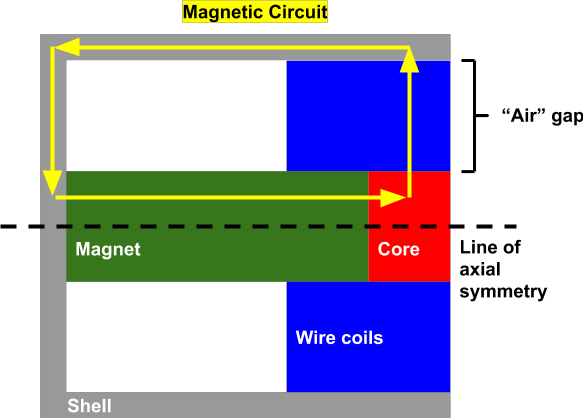
\includegraphics[scale=0.4]{simplifiedMotor.png}
    \caption{Simplified axisymmetric diagram of typical moving-wire voice coil motor}
    \label{fg:simplemotor}
\end{figure}

This means the total reluctance in the circuit can be represented by equation \ref{eq:rttl}, similar to how resistance is calculated in an electrical circuit.

\begin{equation}\label{eq:rttl}
    \mathcal{R}_{total}=\mathcal{R}_{gap}+\mathcal{R}_{mag}+\mathcal{R}_{core}+\mathcal{R}_{shell}
\end{equation}

Magnetic reluctance can be calculated as the proportion of magnetic path length $l_m$ and the product of material permeability $\mu$ and cross-sectional area normal to magnetic flux $A$, seen in equation \ref{eq:rcalc} \cite{coatesTransformerCoresReluctance2018}.

\begin{equation}\label{eq:rcalc}
    \mathcal{R}=\frac{l_m}{\mu A}
\end{equation}

Assuming the shell and core are made out of magnetically conductive material such as mild steel, the permeability of shell and core will be hundreds of times higher than the permeability of "air" gap and magnet \cite{engineeringtoolboxPermeability2016}. Therefore, the reluctance of shell and core can be approximated to zero for the purposes of this calculation.
Substituting simplified equation \ref{eq:rttl} into equation \ref{eq:emmfdef} produces:

\begin{equation}\label{eq:emmfreal}
    \mathcal{F}=(\mathcal{R}_{gap}+\mathcal{R}_{mag})\Phi
\end{equation}

Reluctance between two coaxial cylinders, in this case between the magnet and the shell, can be calculated as in equation \ref{eq:rgap}, assuming all magnetic flux flows through the core \cite{changChapterElectrodynamics2006}. Relative permeability of the gap is approximated to 1 as none of air, silicone or eGaIn are ferromagnetic \cite{engineeringtoolboxPermeability2016}.

\begin{equation}\label{eq:rgap}
    \mathcal{R}_{gap}=\frac{\mu_0 \ln{\frac{r_{out}}{r_{in}}}}{2\pi L_{core}}
\end{equation}

Reluctance through the magnet can be calculated as seen in equation \ref{eq:rmag}, similar to how resistance would be calculated for a cylinder.

\begin{equation}\label{eq:rmag}
    \mathcal{R}_{mag}=\frac{\mu_m L_{mag}}{2\pi r_{mag}^2}
\end{equation}

Substituting equations \ref{eq:rgap}, \ref{eq:rmag} and \ref{eq:emmf1} into equation \ref{eq:emmfreal} gives equation \ref{eq:emmfsubbed} which yields flux in the motor magnetic circuit.

\begin{equation}\label{eq:emmfsubbed}
    \begin{split}
        L_m B_r & = \frac{\ln{\frac{r_{out}}{r_{in}}}}{2\pi L_c}\Phi\\
        \frac{2\pi L_m L_c B_r}{\ln{\frac{r_{out}}{r_{in}}}} & = \Phi\\
    \end{split}
\end{equation}

To calculate the magnetic field density in the "air" gap, which can then be used to calculate force acting on the moving coils, the area of action that the flux is distributed across is also required as seen in equation \ref{eq:fluxdef}.

\begin{equation}\label{eq:fluxdef}
    \Phi = B_{gap}A_{active}
\end{equation}

Substituting equation \ref{eq:fluxdef} into equation \ref{eq:emmfsubbed} gives equation \ref{eq:fluxsubbed}, which can be used to calculate the magnetic field density $B_{gap}$ across the "air" gap.

\begin{equation}\label{eq:fluxsubbed}
    B_{gap} = \frac{2\pi L_{mag} L_{core} B_r}{\ln{\frac{r_{out}}{r_{in}}}A_{active}}
\end{equation}

Using Lorentz's force law substituted with equation \ref{eq:fluxsubbed}, equation \ref{eq:fbil} gives a minimum current $I$ can be obtained given a known required force $F$ and a known length of wire in the magnetic field $L_{active}$.

\begin{equation}\label{eq:fbil}
    \begin{split}
        F & = B_{gap}IL_{active}\\
        I & = \frac{F}{B_{gap}L_{active}}\\
        I & = \frac{F A_{active} \ln{\frac{r_{out}}{r_{in}}}}{2\pi L_{mag} L_{core} B_r L_{active}}
    \end{split}
\end{equation}

The active area in the magnetic field is different for each layer of wire in the motor. Layers of wire further away from the magnet, meaning a larger area and therefore lower magnetic field density. The total active area that magnetic flux is distributed across can be calculated as shown in equation \ref{eq:activearea}, where $n$ is the total number of wire layers. Here the magnet core is assumed to be the same diameter as the magnets.

\begin{equation}\label{eq:activearea}
    A_{active} = \sum_{1}^{n}{A_{active}^{layer}} = 2\pi L_c (r_{core}-r_{wireout} + 2r_{wireout} \frac{(n+1)n}{2})
\end{equation}

The length of wire in the magnetic field can be calculated in a similar fashion, shown in equation \ref{eq:activel}.

\begin{equation}\label{eq:activel}
    L_{active} = L_{core}\pi(layers+1)layers + \frac{L_{core} r_{mag} \pi}{r_{wireOut}}
\end{equation}

Combining equations \ref{eq:fbil}, \ref{eq:activearea} and \ref{eq:activel} yields a final current calculation seen in equation \ref{eq:finalcurrent}.

\begin{equation}\label{eq:finalcurrent}
    I = \frac{F\cdot 2\pi L_c (r_{core}-r_{wireout} + 2r_{wireout} \frac{(n+1)n}{2}) \ln{\frac{r_{out}}{r_{in}}}}{2\pi L_{mag} L_{core} B_r L_{core}\pi(layers+1)layers + \frac{L_{core} r_{mag} \pi}{r_{wireOut}}}
\end{equation}

\subsubsection{Heat and Temperature}

A major challenge for designing electromagnetic motors is coil heat generation, and how to dissipate that heat. Energy is conserved in the motor system, as seen in figure \ref{fg:motorheat}. As a result, power dissipated as heat can be simply calculated using the difference between electrical power input and mechanical power output, assuming no other power is lost from or enters the system.

\begin{figure}[h!]
    \centering
    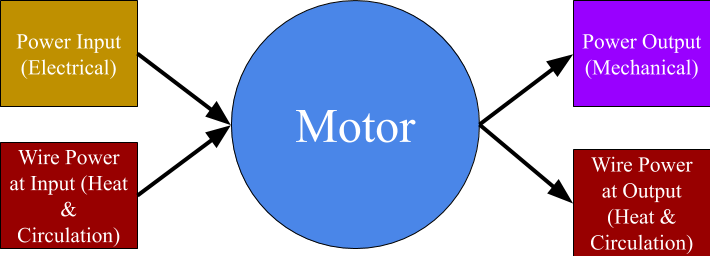
\includegraphics[scale=0.4]{motorheat.png}
    \caption{Conservation of energy in the motor system}
    \label{fg:motorheat}
    \end{figure}
    \begin{equation}\label{eq:pbreakdown}
    P_{in}=P_{out}=P_{mech}+P_{heat}
\end{equation}

Electrical power input is calculated as the product of current and voltage across the motor, or when substituted with Ohm's law becomes the square of current times motor resistance.

\begin{equation}\label{eq:pin}
    P_{in} = IV = I^2R
\end{equation}

Motor resistance can be calculated as a quarter of total wire resistance. This is because in order to create a closed-circuit of tubing to contain eGaIn wires, the whole length of wire effectively becomes two wires in series. This effect is illustrated in figure \ref{fg:parallelwire}. The resistance of two parallel wires each one half the original length is one quarter of the original.

\begin{figure}[h!]
    \centering
    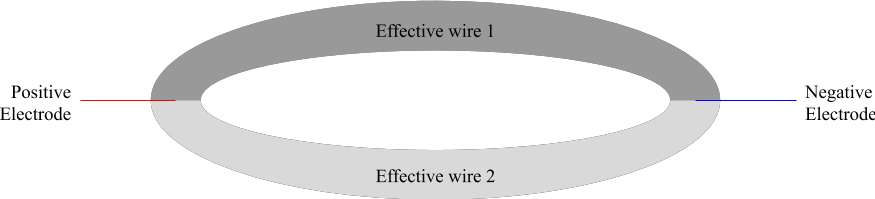
\includegraphics[scale=0.4]{parallelwire.png}
    \caption{Illustration of how a wire circuit causes two effective wires in parallel.}
    \label{fg:parallelwire}
\end{figure}

Wire resistance is calculated via total length of wire divided by cross-sectional area of wire ($A$) and conductance ($\sigma$).

\begin{equation}\label{eq:resistance}
    R=\frac{L_{Wtotal}}{4A\sigma_{eGaIn}}
\end{equation}

Mechanical power output is the dot product of force and displacement per unit time. For a linear motor that travels in one axis only, this simplifies to force times distance per unit time. Force produced by a voice coil motor is equal to the Lorentz force acting on the coils, and distance per unit time is calculated using coil travel distance per cycle multiplied by frequency of cycles. Substituting in the Lorentz force equation and distance calculations, mechanical power can be calculated as seen in equation \ref{eq:pmechbreakdown}.

\begin{equation}\label{eq:pmechbreakdown}
    \begin{split}
   		P_{mech} & = \frac{\textbf{F} \cdot \textbf{x}}{t} \\
    	& = BIL\cdot d_{travel} \cdot f
    \end{split}
\end{equation}

Power dissipated as heat in the wire can be calculated as the difference between power of the wire on input to the system from power on output from the system. Given the wire will a liquid, the power of the wire will be the power in fluid flow, which is the product of flow rate ($Q$), mass density ($\rho$) and energy per unit weight ($c_{pWire}T$). This calculation can be simplified as seen in equation \ref{eq:pheat}.

\begin{equation}\label{eq:pheat}
    \begin{split}
    	P_{heat} & = P_{wireOut} - P_{wireIn} \\
		& = \rho Q c_{pWire} T_{out} - \rho Q c_{pWire} T_{in} \\
		& = \rho Q c_{pWire} \Delta T
    \end{split}
\end{equation}

Combining equations \ref{eq:pin}, \ref{eq:resistance}, \ref{eq:pbreakdown}, \ref{eq:pmechbreakdown} and \ref{eq:pheat} gives a formulation for temperature change of wires, assuming heat energy is conserved in wires. As seen in equation \ref{eq:pheatbreakdown}, this change in temperature is inversely proportional to the flow rate of liquid metal in the motor, assuming liquid that exits the motor can be cooled to input temperature.

\begin{equation}\label{eq:pheatbreakdown}
    \begin{split}
        P_{heat} & = P_{in}-P_{mech}\\
        \rho Q c_{pWire} \Delta T & = \frac{I^2L_{Wtotal}}{A\sigma}-BIL\cdot d \cdot f \\
        \Delta T & = \frac{\frac{I^2L_{Wtotal}}{A\sigma}-BIL\cdot d \cdot f}{\rho Q c_{pWire}}
    \end{split}
\end{equation}

\subsubsection{Liquid Metal Circulation}
To circulate eGaIn through the motor wires a pump has to generate a certain pressure. Assuming the velocity of circulation is slow enough to assume laminar flow, the pressure required to develop a certain rate of flow can be calculated using equation \ref{eq:pressure}.

\begin{equation}\label{eq:pressure}
    P=\frac{8\nu_{eGaIn}L_{Wtotal}Q}{4\pi r_{in}}
\end{equation}

\subsection{Optimisation Algorithm}

\begin{figure}[h!]
    \centering
    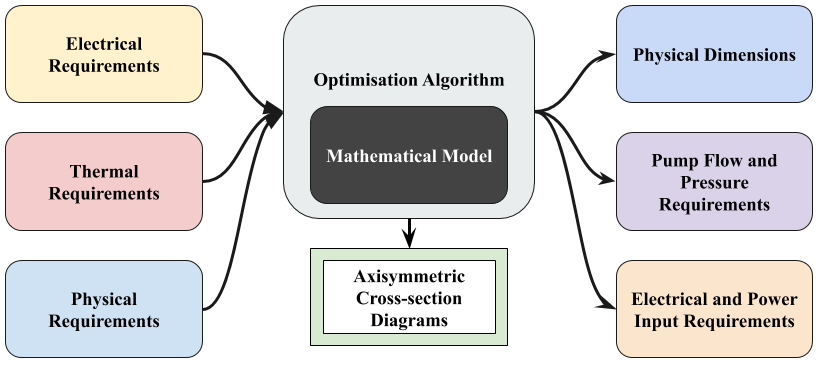
\includegraphics[scale=0.4]{optiAlgro.png}
    \caption{Diagrammatic representation of optimisation algorithm inputs and outputs}
    \label{fg:optiAlgo}
\end{figure}

With the motor reasonably well modelled, it can be optimised to maximise desirable qualities. A grid-search optimisation algorithm was developed to take advantage of the mathematical models outlined in section \ref{section:mm}. Grid search algorithms compare an objective function for every value in a set range of values for each variable. To save time, only designs with even numbered layers of wiring are considered. Designs with odd numbered layers of wiring in the coil introduce additional complications as wiring would need to enter one side of the bobbin and exit the other. One end of the wiring would also need to exit via a hole in the shell, adding difficulty to the design. Every layer is considered separately for the purposes of optimisation, e.g. the optimiser outputs an optimal solution for both 4-layer, 6-layer and 8-layer designs.

As seen in figure \ref{fg:optiAlgo}, the algorithm would only consider solutions that fit certain criteria. The qualifying criteria list with justifications can be found in table \ref{tb:optrequirements}. Solutions that are not compliant are disregarded and the algorithm moves to the next combination of variable values.

\begin{table} [h!]
    \centering
    \caption{List of design requirements and justifications.}
    \label{tb:optrequirements}
    \begin{tabular}{M | M | M}
        \hline
        \textbf{Variable} & \textbf{Requirement} & \textbf{Justification} \\
        \hline\hline
        Output force & Must be over 9 N & Minimum to drive liquid metal pump \\
        \hline
        Acceptable temperature change in wires after circulation & Must be under 30 K & Higher temperatures may be a health and safety hazard \\
        \hline
        Travel distance of motor & Must be over 9 mm & Minimum to drive liquid metal pump \\
        \hline
        Bobbin length & Must be shorter than combined length of core and magnet & Not physically valid otherwise \\
        \hline
        Shell internal diameter & Must be under 80 mm & Not practical for manufacturing, assembly and handling if bigger \\
        \hline
        Total motor current & Must be under 10 A & No power supply available to drive more than 10 A \\
        \hline
        Total volume of wire & Must be under 15 ml & Limit to amount of eGaIn available and difficult to assemble with larger volume \\
        \hline
        Flow rate of liquid metal in wires & Must be positive & Validity check$\dagger$ \\
        \hline
        Electrical power input & Must be positive & Validity check$\dagger$ \\
        \hline
    \end{tabular}
    \\$\dagger$Explicitly stated for sake of the optimisation algorithm.
\end{table}

The variables being optimised for, and the ranges they are optimised for can be seen in table \ref{tb:gridsearch}. These variables were selected as they are independent from one another. All other quantities in the motor are either known requirements, and therefore programmed as constants, or can be derived from these variables.

\begin{table} [h!]
    \centering
    \caption{Grid-search optimisation variables and units.}
    \label{tb:gridsearch}
    \begin{tabular}{c | c | c | c | M}
        \hline
        \textbf{Variable} & \textbf{Units} & \textbf{Minimum} & \textbf{Maximum} &\textbf{Justification} \\ [0.5ex]
        \hline\hline
        Magnet length & m & 5 & 95 & Motor longer than ~100 mm would be unwieldy. Length under 5 mm may be hard to manufacture and assemble.\\
        \hline
        Magnet radius & m & 1 & 20 & Magnets over the diameter of 40 mm  are difficult to purchase commercially and are significant health and safety hazards. \\
        \hline
        Core length & m & 1 & 25 & Reasonable range obtained via trial and error. Under 1 mm may be hard to manufacture and assemble. \\
        \hline
        Bobbin length & m & 5 & 95 & Reasonable range obtained via trial and error. \\
        \hline
    \end{tabular}
\end{table}

The algorithm optimised for a derived variable, the optimisation value $\mathcal{P}$, or product of total motor mass and electrical input power. Total motor mass can be calculated as shown in equation \ref{eq:motormass}. The mass of each component is the volume density of the component material multiplied by component volume. Volume of each component can be obtained using only constants and variables in table \ref{tb:gridsearch}.

\begin{equation}\label{eq:motormass}
    \begin{split}
    	m_{motor} & = m_{shellbase} + m_{shellcylinder} + m_{magnet} + m_{core} + m_{tubes} + m_{wires} \\
    \end{split}
\end{equation}

$\mathcal{P}$ was selected to improve mass efficiency of the motor, to further prevent the motor design from becoming unwieldy in size and mass. Both mass and power expenditure needed to be minimised, and $\mathcal{P}$ encompasses both. Optimisation was conducted assuming the use of 2 mm internal diameter, 3 mm external diameter silicone tubing for wiring. This was the tubing with largest internal volume to total volume ratio that was commercially available.

The optimiser outputted physical dimensions, pump flow and pressure requirements, electrical input requirements and an axisymmetric cross-section diagram to show scale of the optimised motor for each number of layers that the optimisation was run for, which was every even numbered layer up to 14.

As seen in figure \ref{fg:optvariable}, the minimum value of $\mathcal{P}$ increased as the number of wire layers in the motor coil increased. This suggests increases in number of layers and therefore mass generally does not provide enough improvements in power efficiency to be considered effective.

\begin{figure}[h!]
    \centering
    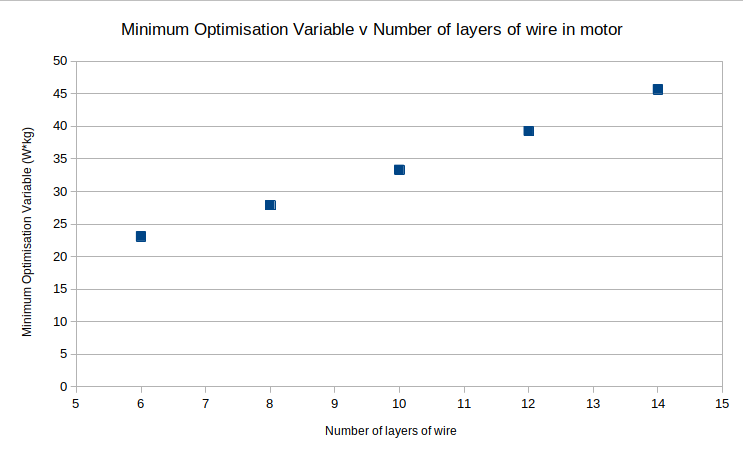
\includegraphics[width=\textwidth]{[P]_v_layers.png}
    \caption{Minimum value of optimisation variable $mathcal{P}$ v number of layers in motor design}
    \label{fg:optvariable}
\end{figure}

The 6-layer solution was selected in the end as there were no valid 2-layer and 4-layer solutions. The optimum 2-layer and 4-layer solutions both required over 10 A of current to output 9 N of force, which was not feasible as the strongest power source available provided a maximum of 10 A. A summary of optimisation outputs can be found in table \ref{tb:optout}. The final design was altered slightly from the optimum output due to component sourcing issues. An axisymmetric cross-section diagram of the final design can be seen in figure \ref{fg:finalmotor}.

\begin{table}[h!]
    \centering
    \caption{Summary of output variables from optimisation algorithm.}
    \label{tb:optout}
    \begin{tabular}{M | l | l | l | l | l | l}
        \hline
        Layer                            & 6  & 8  & 10 & 12 & 14 & Units \\
        \hline\hline
        Magnet Length                    & 42.50 & 50.00 & 57.50 & 65.00 & 72.50 & mm    \\
        \hline
        Magnet Radius                    & 20.00 & 20.00 & 20.00 & 20.00 & 20.00 & mm    \\
        \hline
        Core Length                      & 8.00  & 8.00  & 8.00  & 8.00  & 8.00  & mm    \\
        \hline
        Bobbin Length                    & 24 & 24 & 24 & 24 & 24 & mm    \\
        \hline
        Internal shell radius            & 39.50 & 45.50 & 51.50 & 57.50 & 63.50 & mm    \\
        \hline
        Total wire length                & 9.55  & 13.93 & 18.90 & 24.47 & 30.64 & m     \\
        \hline
        Total wire resistance            & 0.22  & 0.32  & 0.43  & 0.56  & 0.70  & Ohm   \\
        \hline
        Gap field density                & 0.67  & 0.57  & 0.50  & 0.45  & 0.40  & H     \\
        \hline
        Current                          & 8.36  & 6.72  & 5.65  & 4.89  & 4.31  & A     \\
        \hline
        Voltage                          & 1.84  & 2.15  & 2.46  & 2.75  & 3.04  & V     \\
        \hline
        Input power                      & 15.35 & 14.48 & 13.90 & 13.46 & 13.11 & W     \\
        \hline
        Flow to limit temperature change & 0.26  & 0.25  & 0.24  & 0.23  & 0.22  & ml/s  \\
        \hline
        Total mass                       & 1.50  & 1.93  & 2.40  & 2.92  & 3.48  & kg    \\
        \hline
        Optimisation Variable            & 23.07 & 27.89 & 33.32 & 39.26 & 45.66 & W*kg  \\
        \hline
        Pressure Required to drive flow  & 15.39 & 21.15 & 27.53 & 34.49 & 42.03 & kPa  \\
        \hline
    \end{tabular}
\end{table}


\begin{figure}[h!]
    \centering
    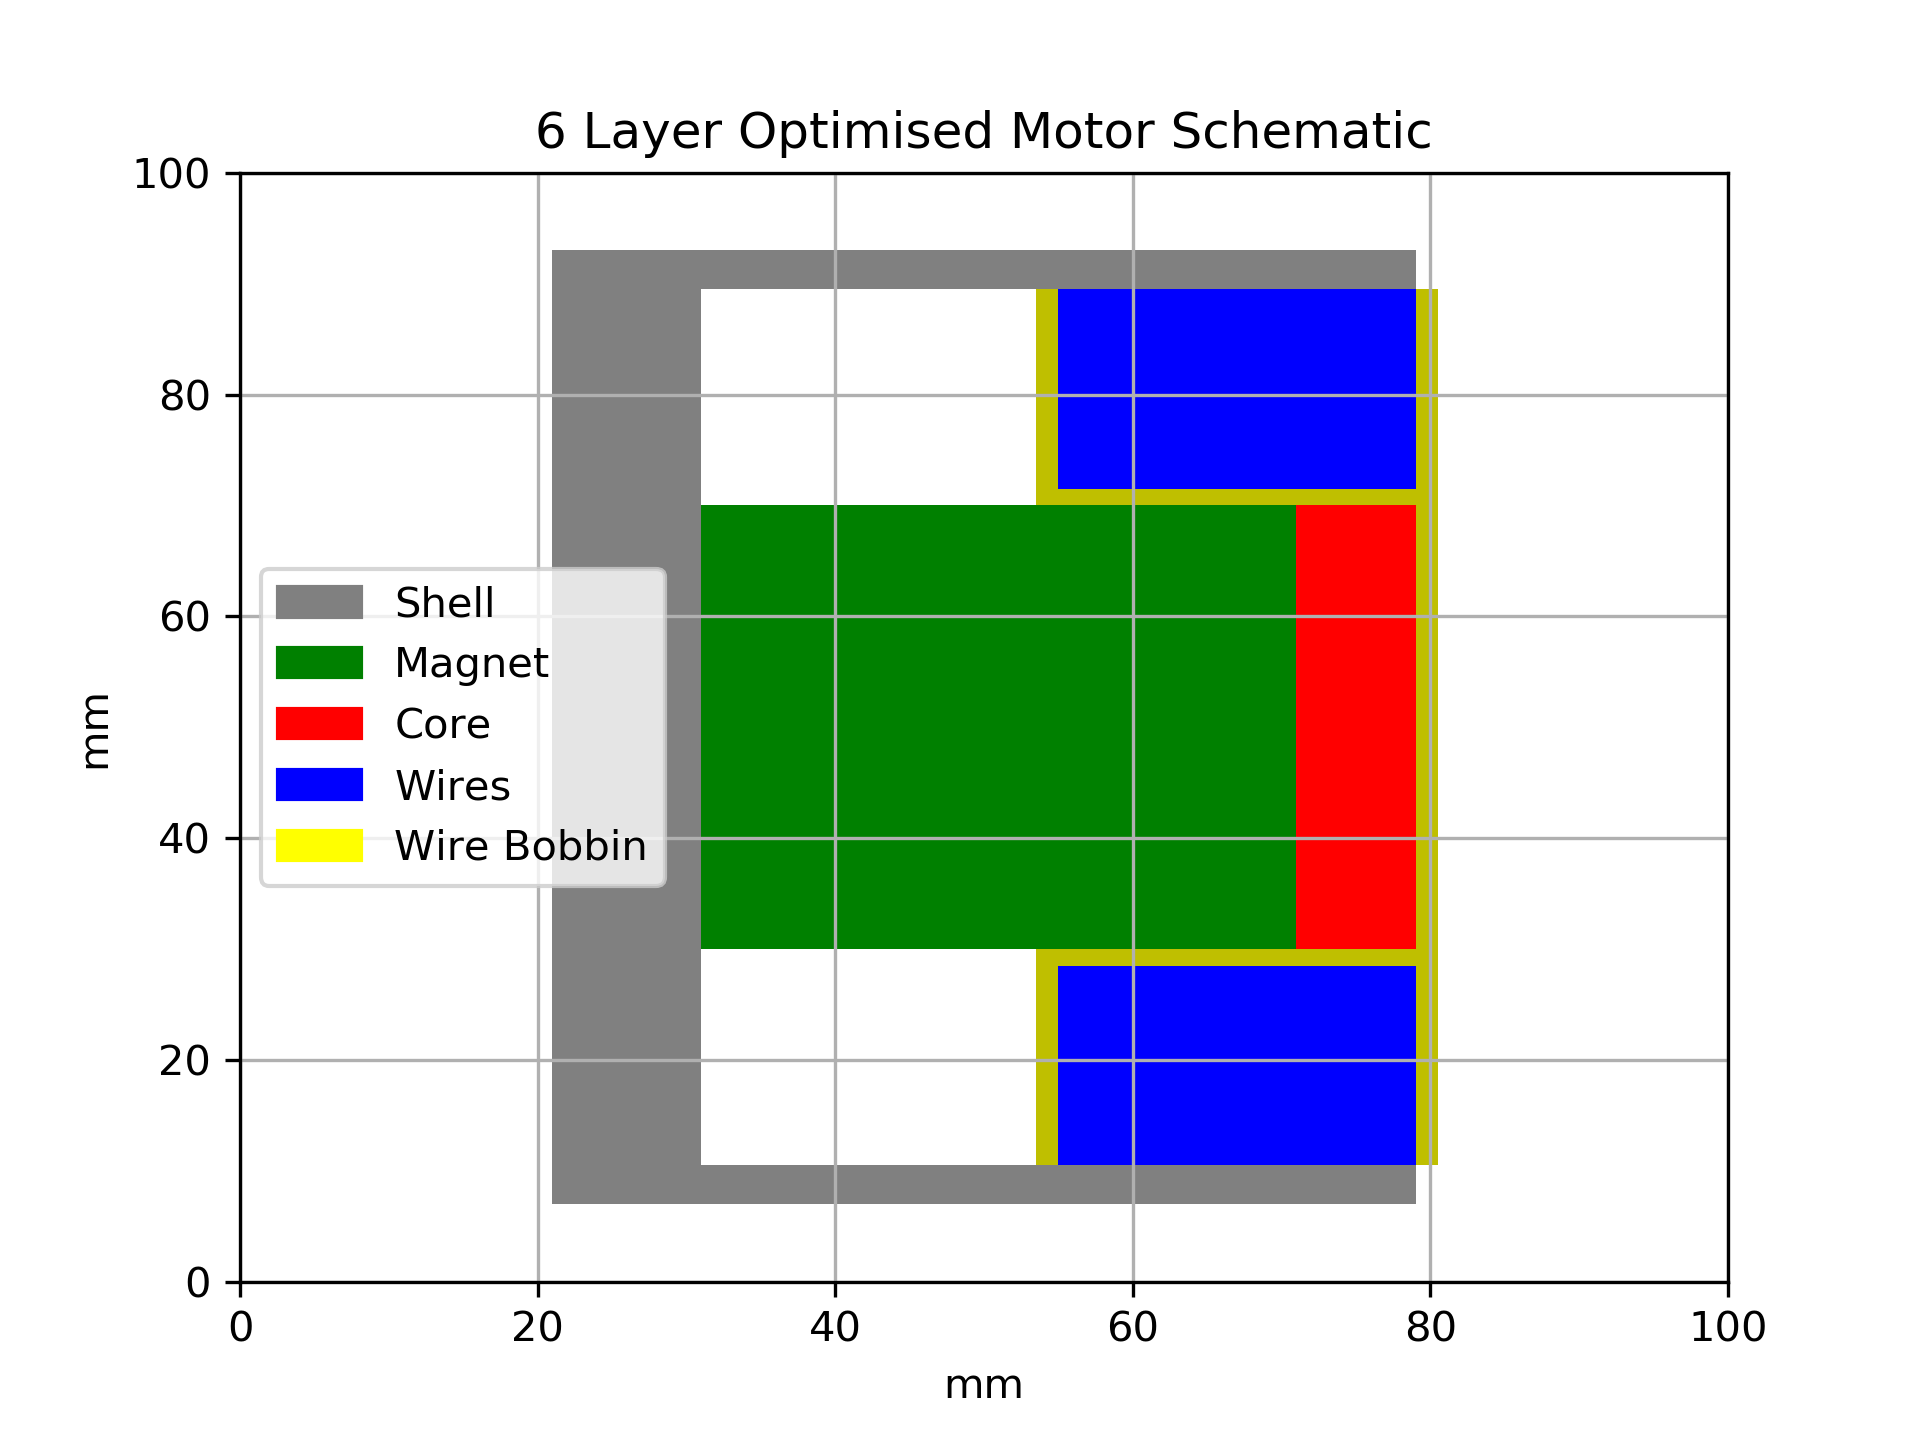
\includegraphics[width=0.5\textwidth]{finalDesign_layers.png}
    \caption{Cross-section diagram of final motor design}
    \label{fg:finalmotor}
\end{figure}

The final motor design features a lightly shorter magnet than the demanded 42.5 mm at 40 mm as no commercially available neodymium magnet supplier sold 42.5 mm long, 40 mm diameter magnets off the shelf. No combination of shorter 40 mm diameter magnets could combine to form a 42.5 mm magnet either. 40 mm length was the closest viable option.

\begin{figure}[h!]
    \centering
    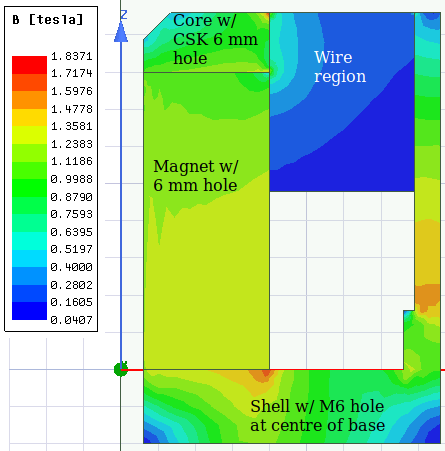
\includegraphics[width=0.5\textwidth]{maxwell.png}
    \caption{Maxwell 2D simulation of magnetic field density in motor}
    \label{fg:maxwellB}
\end{figure}

The final design was verified via finite element analysis using ANSYS Maxwell 2D electromagnetic simulation. The problem was defined as axisymmetric about the z-axis, as seen in figure \ref{fg:maxwellB}. Figure \ref{fg:maxwellB} is a contour plot of magnetic field density B within the motor. This figure validates there is no saturation of magnetic field within the motor, shell or core as maximum field density is under 2 T \cite{mclymanMagneticMaterialsTheir2004}.

\begin{figure}[h!]
    \centering
    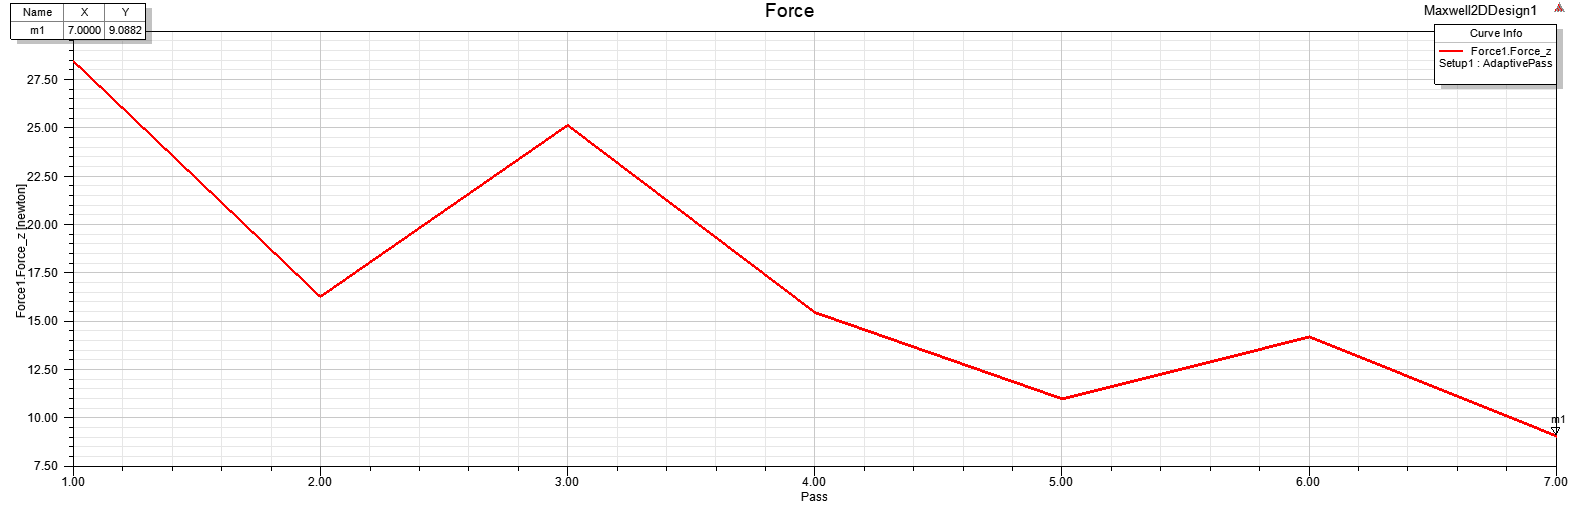
\includegraphics[width=\textwidth]{force.png}
    \caption{Convergence of force on wires to 9.0882 N in Maxwell 2D simulation}
    \label{fg:maxwellforce}
\end{figure}

Convergence of motor force can be seen in figure \ref{fg:maxwellforce}. The force of the motor in the simulation converged at 9.09 N, supporting the notion that calculations in section \ref{section:mm} are correct.

\subsection{Physical Design and Manufacturing}

Due to purchasing constraints, 4 axial, 40 mm diameter, 10 mm tall N45 grade neodymium disc magnets were used in series to substitute for the required 40 mm tall cylinder magnet. The disc magnets also come with countersunk unthreaded M6 holes for fastening.

\subsubsection{Shell}

The shell of the final motor features a two-piece design composed of a shell cylinder and shell base. This was done to ensure safe assembly of magnets into motor by allowing the assembly of magnets onto base via sliding. The 40 mm diameter N45 magnets were difficultly strong, and would shatter if allowed to accelerate into the shell. Accelerating magnets of that strength were also deemed to be a health and safety hazard.

\begin{figure}[h!]
    \centering
    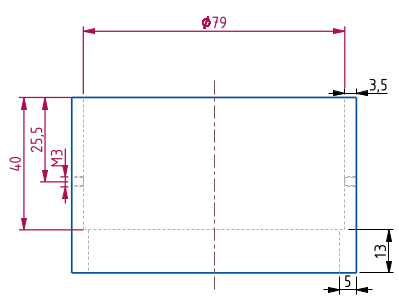
\includegraphics[scale=0.5]{shellcylinder.png}
    \caption{Axisymmetric cross-section drawing of final shell cylinder}
    \label{fg:shellcylinder}
\end{figure}

The shell was made 3.5 mm thick in most part to avoid magnetic saturation within the shell. A 13 mm, 5 mm thick region of the shell cylinder towards the base, seen in figure \ref{fg:shellcylinder}, was made to more comfortably interface with the shell base. Manufacturing constraints meant that the lathe finish on both cylinder and base were not perfect, and a wider interface could help prevent contact issues.

Threaded M3 holes normal to the surface of the shell were made 25.5 mm from the top. These holes were used to secure shell cylinder while base, magnets and core were lowered onto to the cylinder. For more information on this step see section \ref{section:shellassembly}.

A threaded M6 hole, seen in figure \ref{fg:shellbase}, was implemented at the centre of the shell base for the magnets and core to securely bolt onto. Four unthreaded M3 holes were made through the shell base for bolts that secure the assembly spacer to travel through, and also enable ventilation while motor is in operation. For more information on the assembly spacer see section \ref{section:shellassembly}.

Both shell base and cylinder were turned on a lathe from 1020 grade 100 mm diameter engineering bar steel stock.

\begin{figure}[h!]
    \centering
    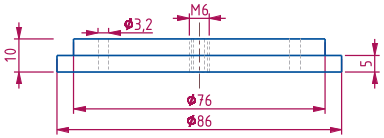
\includegraphics[scale=0.5]{shellbase.png}
    \caption{Axisymmetric cross-section drawing of final shell base. Units in mm.}
    \label{fg:shellbase}
\end{figure}

\subsubsection{Core}

The core of the motor is a 8 mm thick, 40 mm diameter cylinder with countersunk unthreaded M6 hole in the centre. The hole in the centre allows for a bolt to travel through magnets and affix both core and magnets to the shell base.

\begin{figure}[h!]
    \centering
    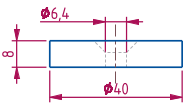
\includegraphics[scale=0.5]{core.png}
    \caption{Axisymmetric cross-section drawing of final core. Units in mm.}
    \label{fg:core}
\end{figure}

\subsubsection{Wire Bobbin}

The wire bobbin was the most physically complex part in the final motor. The bobbin had to travel with the wires, translate force from the wires to an interface, and guide wire winding.

To achieve these requirements, several design features were incorporated. Feature 1 of figure \ref{fg:bobbin} shows the body of the bobbin contains guide threads for winding the first layer of tube. Feature 2 are slits that follow the shape of the thread and allow wire to enter and exit the bobbin. There is one entry and one exit in each slit. Feature 3 shows the "nozzle" interface of the bobbin, used to connect to the load. The nozzle shape adds additional structural integrity as the interface bolt may move. The interface was defined here as an M3 bolt, and the nozzle features an unthreaded M3 hole. On the other side of the M3 hole is feature 4, a hexagonal M3 nut shaped slot allows a nut to secure the bolt without rotating. Feature 5 shows flanged end-plates on the bobbin to provide strength to the force-bearing parts of the bobbin while maintaining lower weight.

Due to the required complexity of the bobbin, it had to be SLA 3D printed. The printing was done on a Formlabs Form 2 printer and post-processed on Formlabs Form Wash and Form Cure processors. The print was made using Formlabs High Temperature resin, as that was the only resin that would withstand 50 \degree C comfortably. 50 \degree C represented the a 30 K temperature change specified in the design requirements from room temperature of about 20 \degree C. Feature 6 of figure \ref{fg:bobbin} are holes to prevent cupping of the part during printing, and also have the added benefit of equalising pressure during bobbin movement.

\begin{figure}[h!]
    \centering
    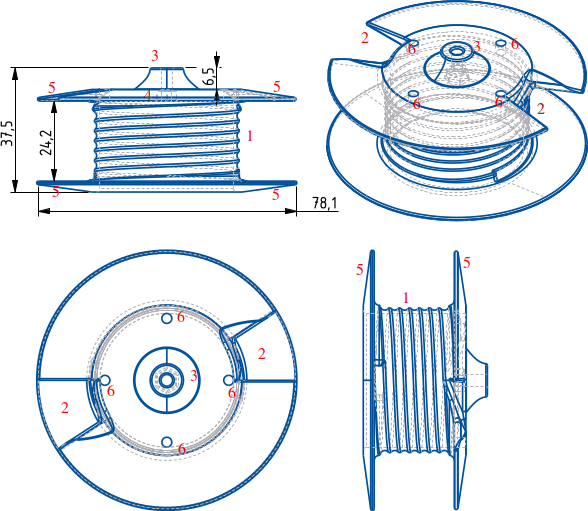
\includegraphics[scale=0.5]{bobbin.png}
    \caption{Three-view drawing of final wire bobbin. Units in mm. Annotations in red.}
    \label{fg:bobbin}
\end{figure}

\subsection{Assembly}

\subsubsection{Shell and Magnet Assembly} \label{section:shellassembly}

\begin{figure}[h!]
    \centering
    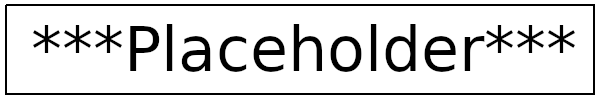
\includegraphics[width=0.5\textwidth]{placeholder.png}
    \caption{Contraption used to safely assemble magnets and core onto shell base.}
    \label{fg:assemblingmagnet}
\end{figure}

Tooling was required to assemble the motor magnets and shell due to strength and size of the magnets. The tool set shown in figure \ref{fg:assemblingmagnet} allows magnets and core to slide into position. Each layer of the tool is the same height as a magnet, and a layer is added each time a magnet is installed. The round sliding tool was used to prevent magnets from flying off the platform tool onto other magnets while it was sliding.

After the magnets and core were installed onto the base and bolted secure, a spacer shown in figure \ref{fg:spacer} was also bolted onto the shell base. The purpose of the spacer was to ensure during assembly of shell base to cylinder magnets did not stick to the cylinder. The spacer was turned from polyethylene stock on a lathe and then tapped with threaded M3 holes that aligned with ones on the shell base.

\begin{figure}[h!]
    \centering
    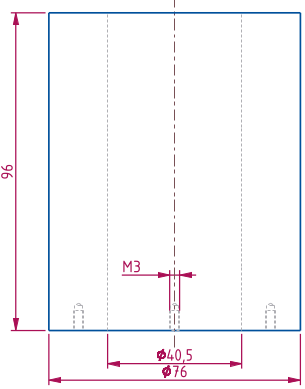
\includegraphics[width=0.3\textwidth]{spacer.png}
    \caption{Spacer used in assembly of shell base to shell cylinder.}
    \label{fg:spacer}
\end{figure}

The base, magnets, core and spacer were then lowered onto the cylinder using a pulley. This process is illustrated in figure \ref{fg:assemblingshell}. An eyebolt was attached to the base and suspended using steel rope. As the white spacer is longer than the cylinder, a tool that accepted the excess length was needed. The Cylinder is bolted onto the tool using L-fixtures, and the tool was bar-clamped onto the underside of an aluminium door frame. The pulley was attached to the top side of that door frame. The door was attached to a non-magnetic room that used to house an MRI machine. The assembled shell, magnets and core can be seen in figure \ref{fg:assembledshell}.

\begin{figure}[h!]
    \centering
    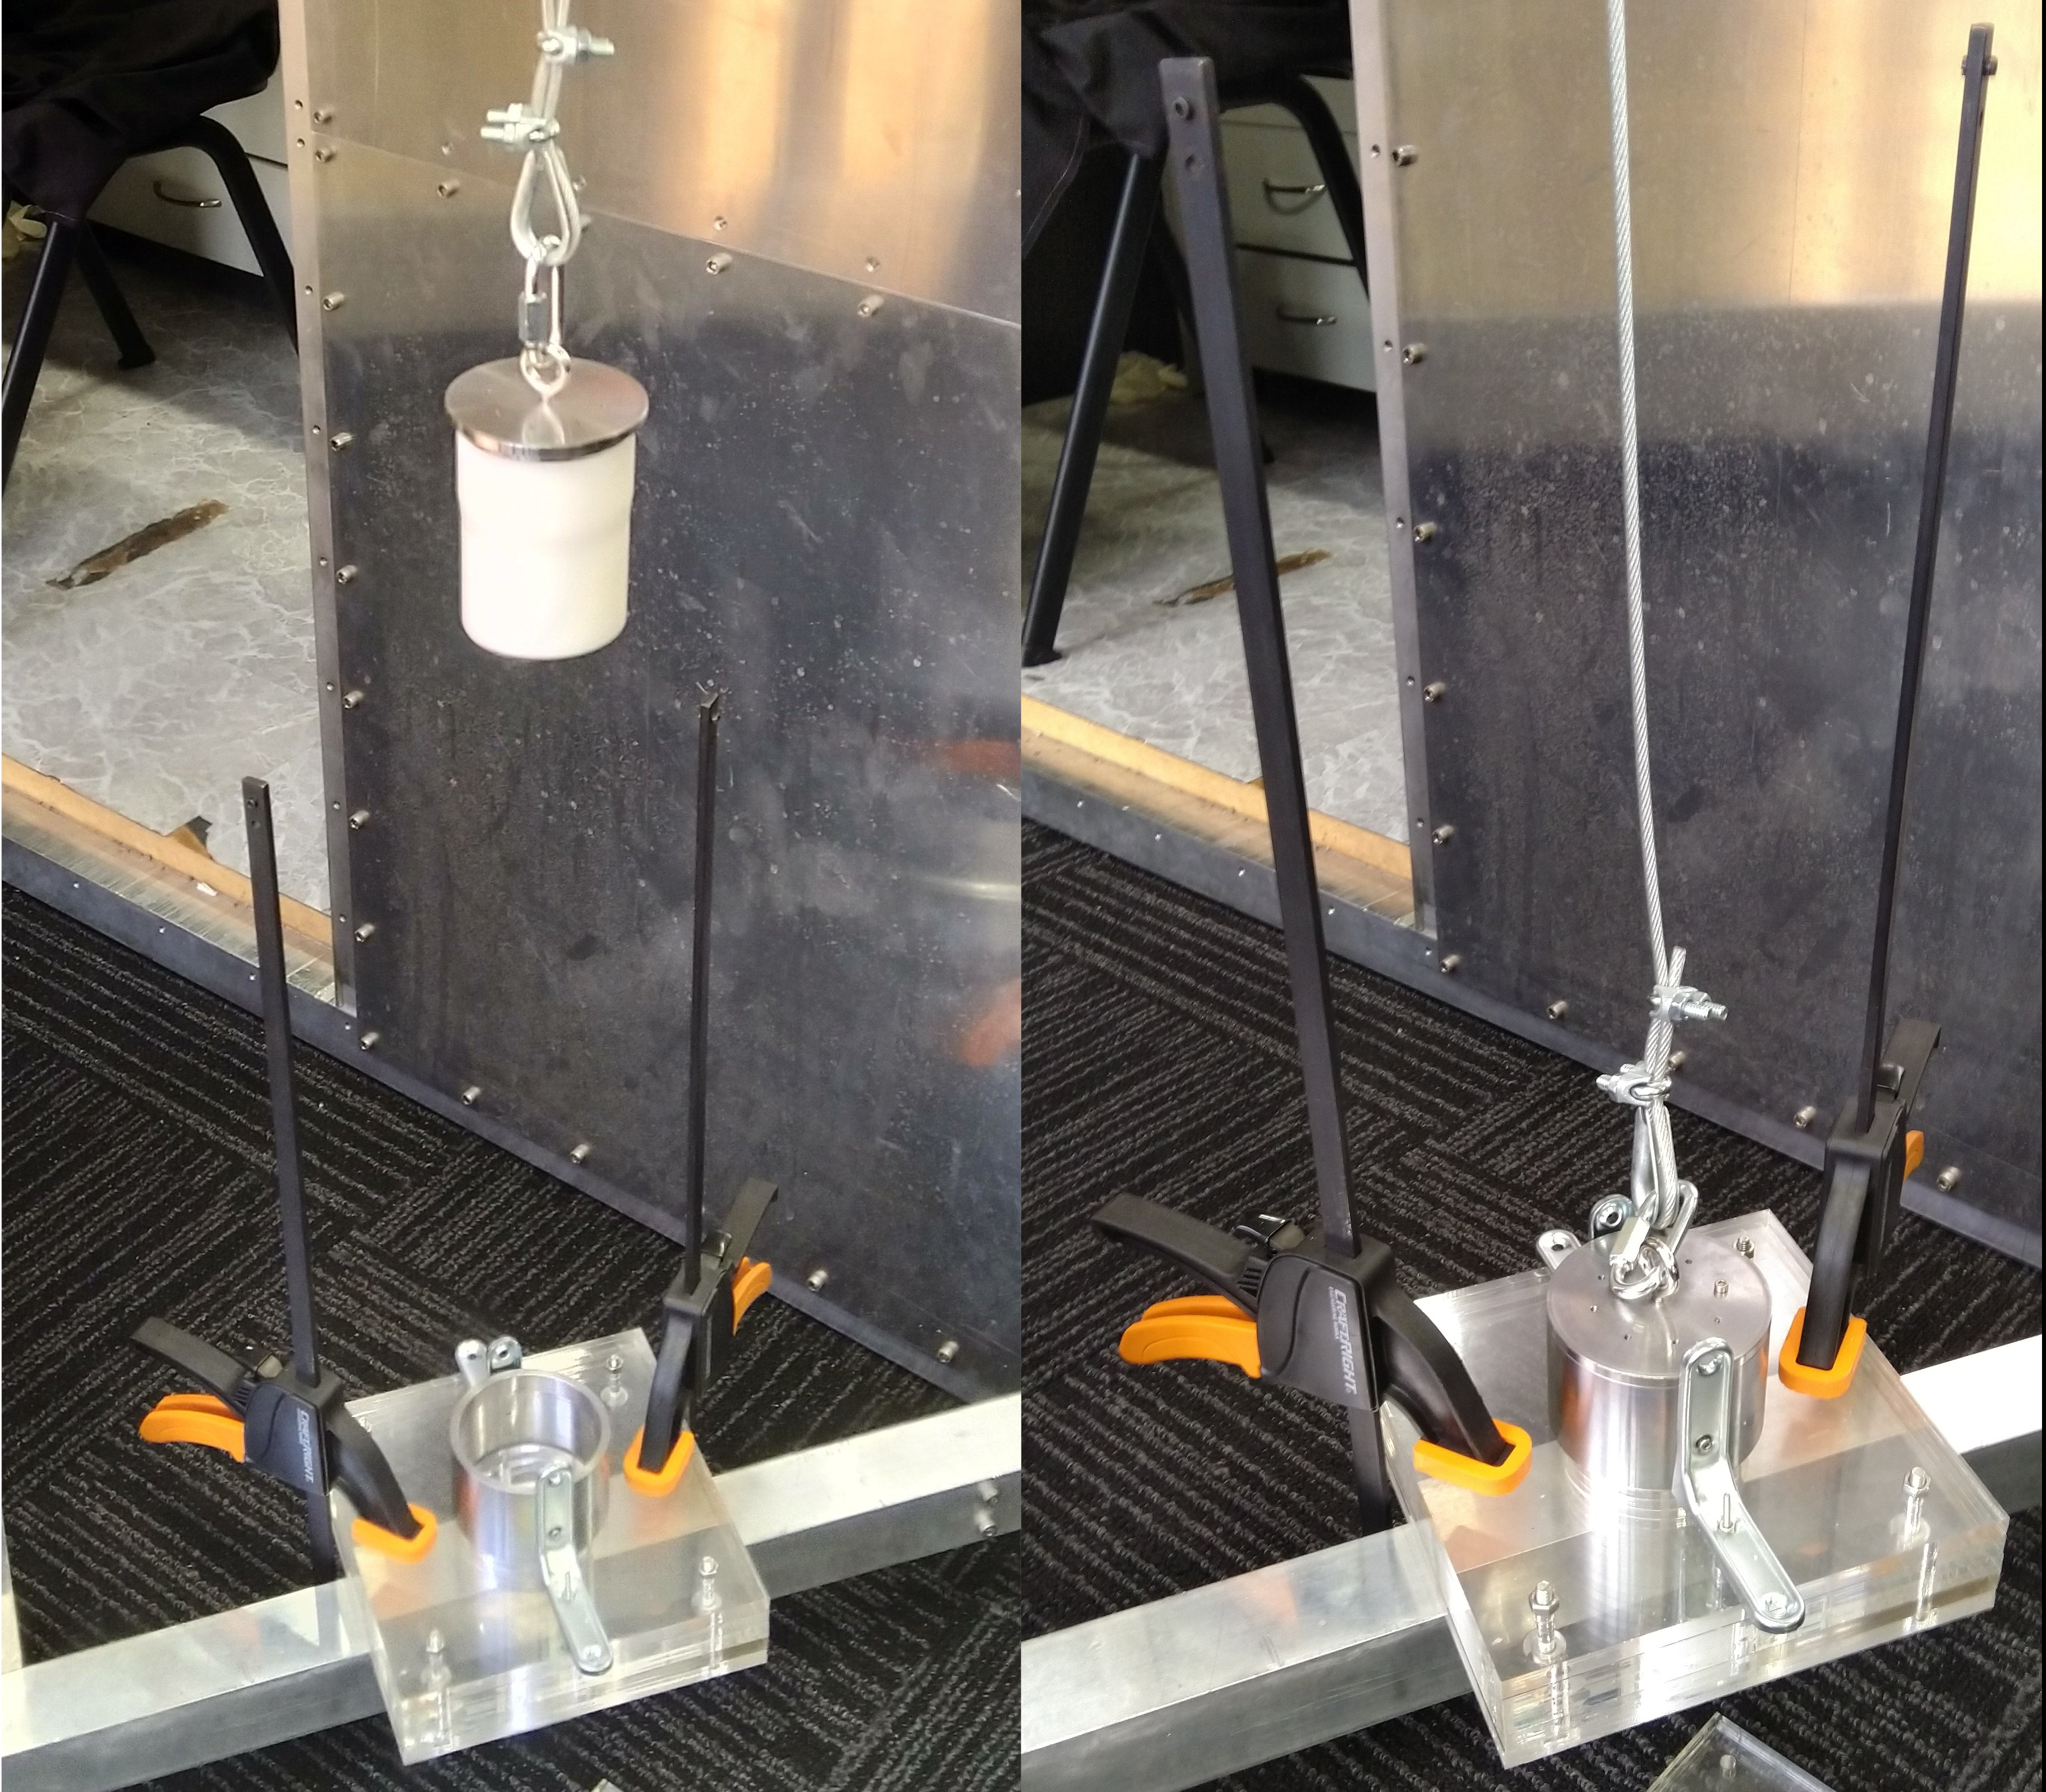
\includegraphics[width=0.5\textwidth]{assemblingshell.png}
    \caption{Shell base with magnets and core attached being lowered onto shell cylinder.}
    \label{fg:assemblingshell}
\end{figure}

\begin{figure}[h!]
    \centering
    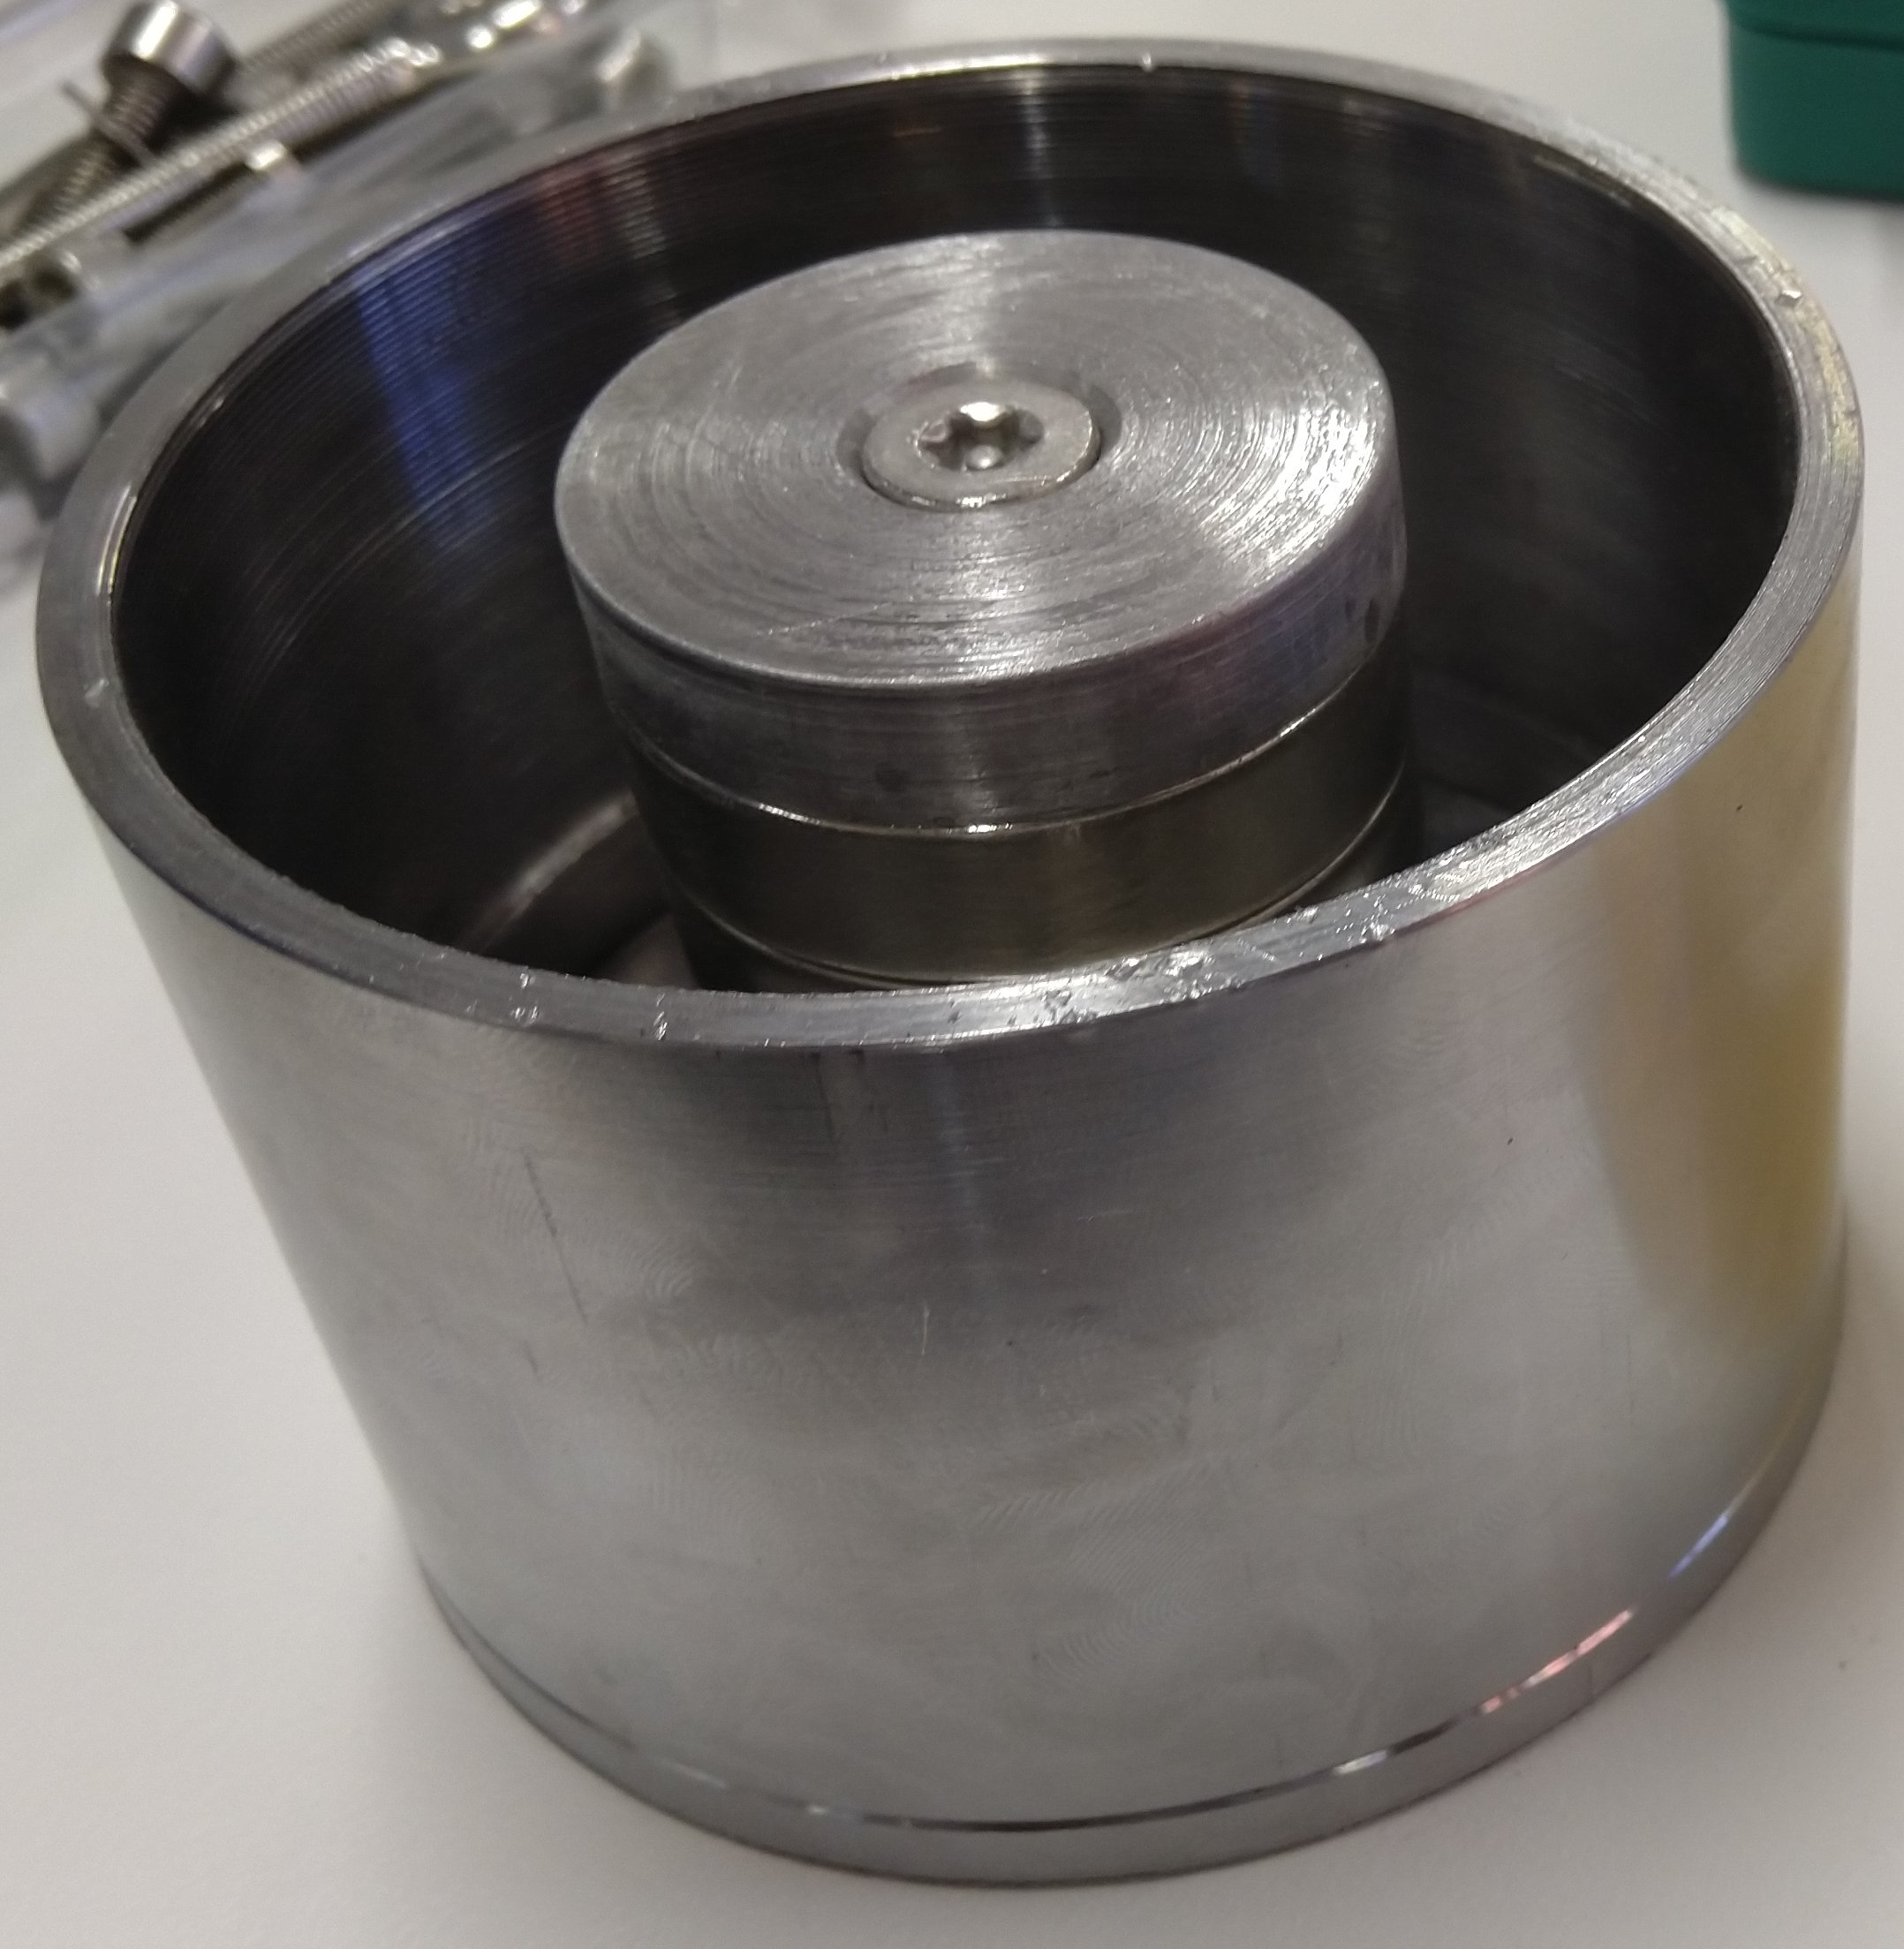
\includegraphics[width=0.5\textwidth]{assembledshell.jpg}
    \caption{Assembled shell with magnets and core attached.}
    \label{fg:assembledshell}
\end{figure}

\subsubsection{Wire Assembly}

After the bobbin was printed and post-processed, silicone tubing was wound across the part. Two parallel strands of tubing, representing the two effective wires of the motor, were wound, one entering and exiting at each slit. This process was done by hand, and every care was taken to avoid kinking, stretching and squeezing of tubes. The winding process was restarted every time one of the issues above were encountered. A photo of the complete wound bobbin before eGaIn was injected can be seen in figure \ref{fg:assembledbobbin}. A total 7.25 m of silicone tubing was used in the bobbin, including the loose ends, as evidenced by 12.75 m tubing left from a 20 m package. This is 2.25 m shorter than designed. The discrepancy was likely to have been caused by the silicone tube stretching during winding, meaning there was less silicone tube wound over the same distance.

\begin{figure}[h!]
    \centering
    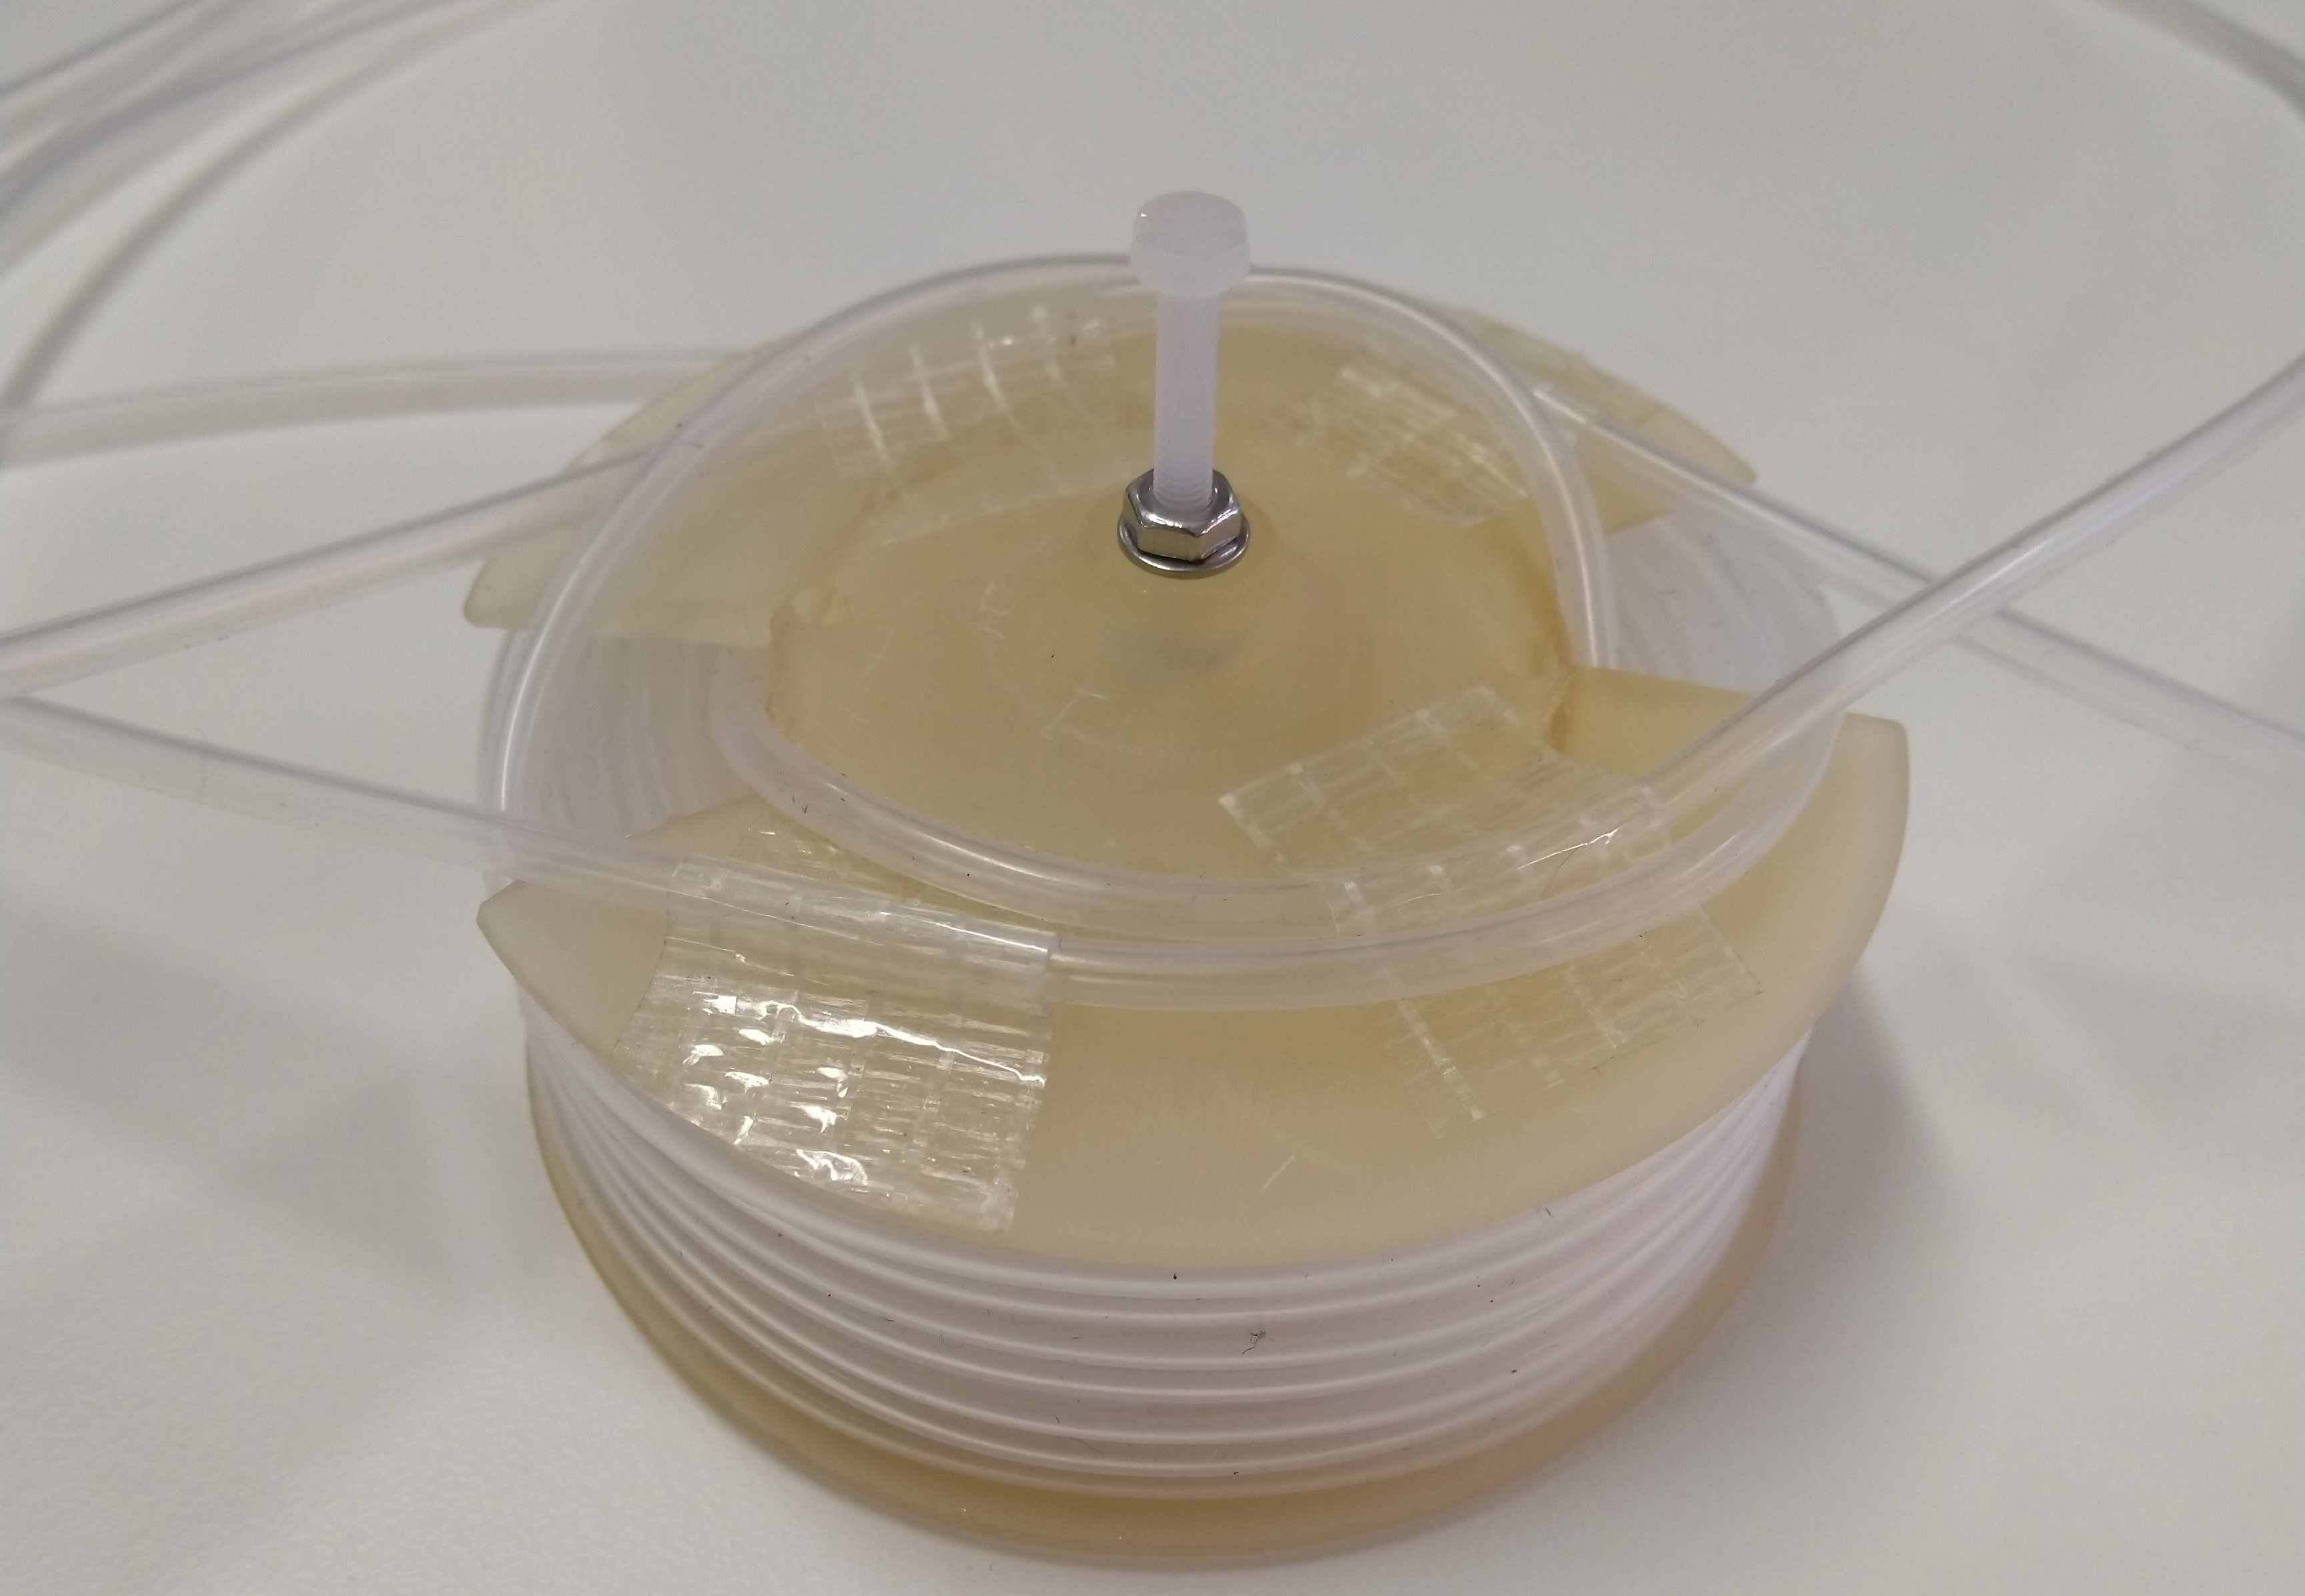
\includegraphics[width=0.5\textwidth]{assembledbobbin.jpg}
    \caption{Bobbin with complete silicone tube windings. Tubes wound by hand.}
    \label{fg:assembledbobbin}
\end{figure}

eGaIn was injected into the tubing from via the reservoir using a 60 ml syringe with a tapered tip. A pipette was used to transfer eGaIn from its container into the syringe, as shown in figure \ref{fg:injectsyringe}. 266.57 g or 42.65 ml of eGaIn was dispensed, including in the tubing, the reservoir and a small spillage. This was discerned via weighing the bottle of eGaIn before and after dispensation. The expected volume of liquid inside 7.25 m of 2 mm internal diameter tubing is 22.78 ml. Even accounting for the loose wire at the ends, rounding up to 8 m of wire there would only be 25.13 ml of volume. The dispensed amount is equivalent to the volume of 8 m of 2.73 mm internal diameter tubing. This may have been caused by stretching of silicone tubing during filling of eGaIn, increasing the average diameter of the tubes. If this is the case, the fill factor of the coils may have increased, potentially improving the possible efficiency of the motor.

\begin{figure}[h!]
    \centering
    \includegraphics[width=0.5\textwidth]{injectegain.jpg}
    \caption{Photo of eGaIn filling in process. Pipette and syringe can be seen with motor in fish bin.}
    \label{fg:injectsyringe}
\end{figure}

Two electrodes were then attached to the ends of effective wires in the motor. One electrode was made using a barbed T-fitting, and the other was three layers of laser-cut acrylic glued together that acts as an open-air reservoir. The reservoir had four holes: two at the bottom for connecting with silicone tubing, one at the top of the side for ventilation and facilitate controlled overflow, and one at the top that can be used to inject eGaIn into the tubing. This was also the hole the electrode was placed. Both electrodes were made of tungsten carbide, which is not known to corrode via eGaIn \cite{indiumcorporationPRODUCTDATASHEET2019}. The motor was then bolted to an L-shaped acrylic support structure that secures both electrodes. The reservoir was superglued onto the side of the support structure, and excess tubing were tape secured onto the support structure. The assembled motor before eGaIn was injected can be seen in figure \ref{fg:jignoegain}.

\begin{figure}[h!]
    \centering
    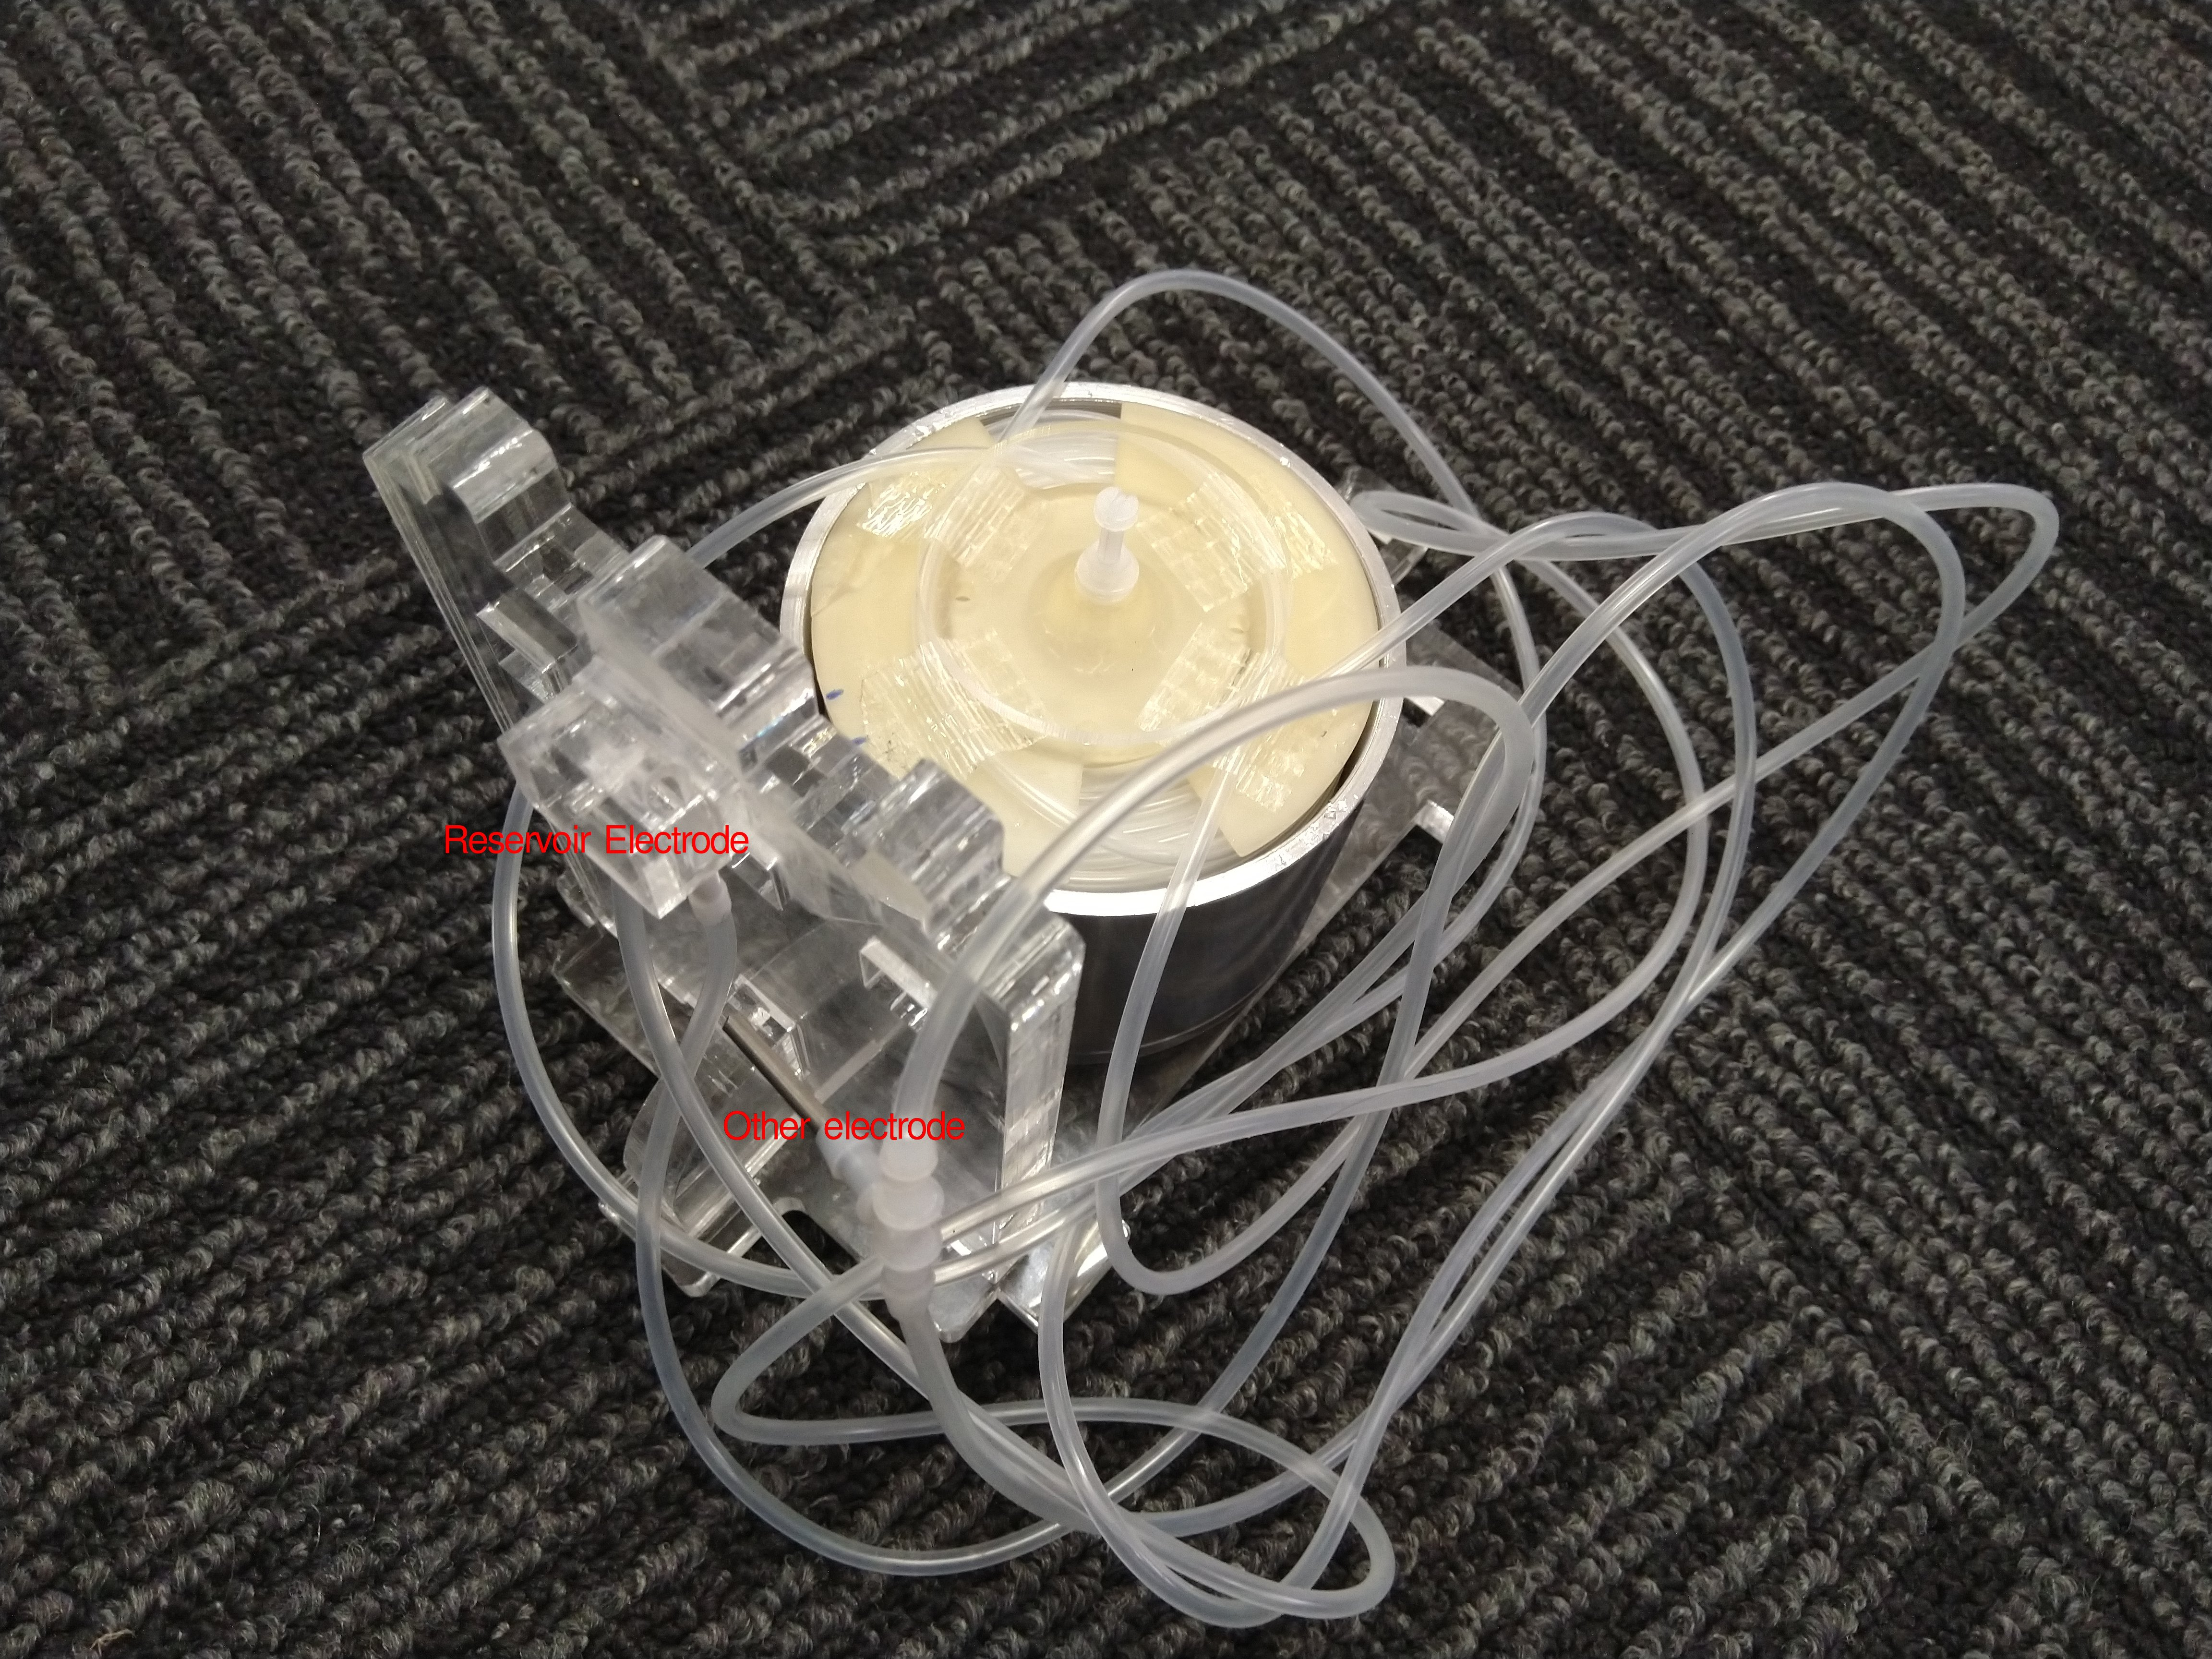
\includegraphics[width=0.5\textwidth]{jignoegain.jpg}
    \caption{Complete motor assembly prior to eGaIn injection.}
    \label{fg:jignoegain}
\end{figure}

The assembled motor was then transferred into a fish bin, where the support structure was taped to the bottom.

\subsubsection{Health, Safety and Containment}

Gallium, indium and eGaIn are not toxic to touch, but can potentially cause harm if ingested or inhaled \cite{dickeyEutecticGalliumIndiumEGaIn2008}. However, eGaIn is known to be corrosive towards most solid metals including iron, copper and aluminium alloys \cite{cuiLiquidMetalCorrosion2018}. In particular, without specific surface treatment, aluminium parts in the lab may corrode rapidly on contact with eGaIn. The contamination and corrosion of eGaIn was minimised via containment procedures outlined in table \ref{tb:safety}.

\begin{table} [h!]
    \centering
    \caption{Safety procedures for handling eGaIn.}
    \label{tb:safety}
    \begin{tabular}{L | L}
        \hline
        \textbf{Procedure} & \textbf{Justification} \\ [0.5ex]
        \hline\hline
        Fish bin contains all eGaIn & Contains spillage and splattering \\
        \hline
        Gloves on any time operating in fish bin & Make sure eGaIn does not leave on skin of hand\\
        \hline
        Disposable cup under both electrodes & Avoid issues with overflowing and tube disconnecting \\
        \hline
        Lid on fish bin at all times when not actively operating in bin & Contains tipping and splattering \\
        \hline
        Goggles on at all times when around fish bin and lid is off & Protect against injury from motor and eGaIn splatter \\
        \hline
        Check connection integrity and temperature before activating motor & Avoid connection failures \\
        \hline
        Check hands and clothes after taking gloves off & Avoid contamination due to broken gloves \\
        \hline
    \end{tabular}
\end{table}

\newpage

\section{Force Characterisation}

\subsection{Method}

The motor is oriented vertically, and drives a cup that contains a known mass of weights. The motor interfaces with the cup via an M3 screw through the bobbin and bolted to a 3.5 mm hole drilled at the centre of the cup base. Another cup of the same size is used to hold the weights for convenient placement and removal. Each plastic cup has a mass of 8.05 g. Weights used are "3oz" lead fishing reef sinkers, which are dense and non-ferromagnetic. The weights were individually weighed, labelled and recorded. One sinker weight is added at a time. Current supplied to the motor is decreased until there is no longer enough force to balance gravity force of the sinkers. Due to a lack of bearings in the motor design, sometimes the bobbin gets caught on the core or the shell. A gentle wiggle of the bobbin usually fixes the problem. The current is decreased because the bobbin appears more likely to be caught when the cups are closer to the core. This setup can be seen in figure \ref{fg:forceexperiment}.

\begin{figure}[h!]
    \centering
    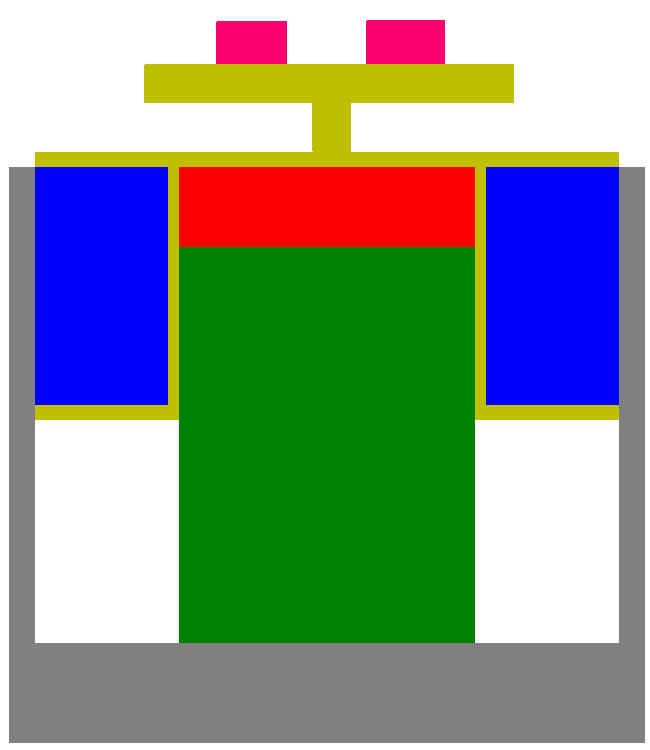
\includegraphics[width=0.5\textwidth]{forceexperiment.jpg}
    \caption{Experiment setup to characterise force output of motor given different electrical input.}
    \label{fg:forceexperiment}
\end{figure}

\subsection{Results}

Results from the experiment suggests the motor has a linear current-force response between 4 A and 10 A current input, seen on figure \ref{fg:forceplot}. This is the expected response from a voice coil motor. This also means power increases exponentially as force and current increases, and therefore the motor is more power-efficient at lower currents.

\begin{figure}[h!]
    \centering
    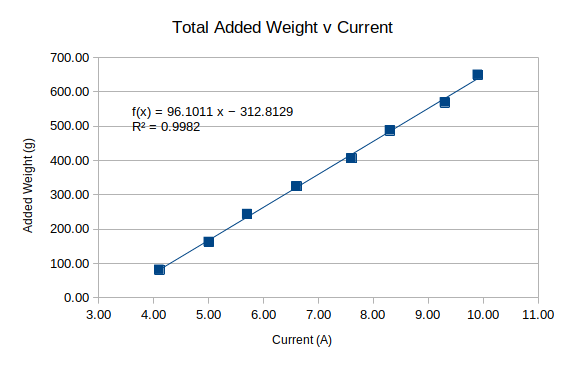
\includegraphics[width=\textwidth]{resultforcevcurrent.png}
    \caption{Total added weight plotted against provided current. Y-intercept provides an estimate for true bobbin mass.}
    \label{fg:forceplot}
\end{figure}

Using the line of best fit in figure \ref{fg:forceplot} the effective mass of the bobbin can be extrapolated using the y-intercept of the line. The effective mass of the bobbin is approximately 312 g, lower than the sum of the liquid and solid parts that went into the bobbin, at approximately 260 g and 80 g respectively. This is likely because of the loose wire not moving with the bobbin, the eGaIn in those parts of wire, eGaIn in the reservoir. The small spill also contributed to the total dispensed mass of eGaIn.

\begin{table}[h!]
    \centering
    \caption{Analysis of force experiment results.}
    \label{tb:fullresults3}
    \begin{tabular}{ L | l | l }
        \hline
        Item & Value & Units \\
        \hline\hline
        Average efficiency ex. Bobbin & 1.00 & $NA^{-1}$ \\
        \hline
        Mass of bobbin \& fixed cup & 335.22 & g \\
        \hline
        Current required for 9 N & 8.75 & A \\
        \hline
        Theoretical calculated current for 9 N & 8.50 & A \\
        \hline
    \end{tabular}
\end{table}

The final motor showed very similar properties to theoretical calculations. Despite seemingly containing a lot more eGaIn, the motor required similar current to output the target force of 9 N, as compared in table \ref{tb:fullresults3}.

\newpage

\section{Discussion}
This project successfully demonstrated proof-of-concept for using liquid metal as the conductor in an electromagnetic motor. The motor was functional, used non-rigid wires that conduct using liquid eGaIn and had very similar efficiency as modelled. The motor also had incorporated in its design, albeit untested, the ability to circulate liquid metal in its coils for cooling. The above design provides a good foundation for future studies that wish to explore electromagnetic motors that use liquid metal in coils, or for cooling those coils by circulating the metal.

The motor also demonstrates a significant limitation of using eGaIn as a conductor - the motor design was not particularly efficient. Had the eGaIn in the final motor design been substituted for a more conductive material such as copper, the motor would have been much more efficient. A motor of the same size filled with copper coils of the same diameter threaded through the same silicone tubing instead of eGaIn will consume under 12\% of the power to produce the same force output. If the volume of the wiring was substituted entirely for 0.22 mm diameter copper wire, a common type of wire used for electromagnetic motors of this force scale, the motor would draw under 28\% of the original power to produce the same force, and require only 6.2\% of the current, both seen in table \ref{tb:coppercompare}. eGaIn coiled motors will inherently have poor energy efficiency as a result, but not necessarily an order of magnitude poorer than other conductors as their resistivity difference would suggest.
\begin{table}[h!]
    \centering
    \caption{Comparison between final eGaIn motor and two hypothetical solutions using copper wiring.}
    \label{tb:coppercompare}
    \begin{tabular}{S | c | c | c | c}
        \hline
        \textbf{Variable} & \textbf{eGaIn solution} & \textbf{Copper equal} & \textbf{Copper fill} & \textbf{Units} \\ [0.5ex]
        \hline\hline
        Total wire length & 9.55 & 9.55 & 157.76 & $m$ \\
        \hline
        Total wire resistance & 0.22 & 0.026 & 17.11 & $\Omega$ \\
        \hline
        Required current & 8.5 & 8.5 & 0.51 & $A$ \\
        \hline
        Power & 15.90 & 1.88 & 4.45 & $W$ \\
        \hline
        Current-Force Efficiency & 1.06 & 1.06 & 17.64 & $NA^{-1}$ \\
        \hline
        Power-Force Efficiency & 0.57 & 4.79 & 2.02 & $NW^{-1}$ \\
        \hline
    \end{tabular}
\end{table}

The liquid nature of the coil material also poses a challenge to the motor's efficiency. Tubing is required to encase the liquid metal and resist any pressure by the liquid due to circulation flow or even gravity. The silicone tubing used for this design, $3\ mm$ outer diameter and $2\ mm$ inner diameter, had the higher internal to external volume ratio of commercially available silicone tubing at 0.44. Most other commercially available tubing having ratios 0.2 or lower, such as the $5\ mm$ outer diameter, $2\ mm$ inner diameter that was sent to the lab by mistake. This means with tubing, the highest possible fill factor of the coil is 0.44, assuming the space is perfectly occupied by tubing. This represents a large discount on possible volume efficiency of the motor, and presents challenges for miniaturisation of the motor design.

\begin{equation}\label{eq:fbil2}
    F = BIL_{active}
\end{equation}

The motor was also quite heavy due to large and strong magnets it required. A longer magnet meant more magnetic flux can be expected in the circuit, and a larger diameter magnet meant a better active magnetic circuit gap area $A_{active}$ to active wire length $L_{active}$ ratio. A larger active area means lower magnetic flux density $B$, which decreases Lorentz force, and higher active length means a higher Lorentz force as per the Lorentz force shown in equation \ref{eq:fbil2}. Miniaturisation of any motor design will also need to contend with this challenge that will decrease the efficiency of smaller motors.

The limitations of eGaIn meant stronger magnets were required to generate the target force with reasonable current input. Having strong magnets also meant needing a thicker shell to avoid magnetic field saturation. The current design saw magnetic field density peak at 1.8 T in the shell wall, while even high permeability steel can expect to saturate between 1.6 and 2.2 T \cite{laughtonElectricalEngineerReference2002}. Steel is quite dense and contributed the most to the mass of the motor.

****************** You need to balance flow and resistance. larger tube means better flow and smaller resistance - really low voltage, high current. *************************

There were some interesting heat properties observed in the motor during testing. The barbed T-junction electrode was the fastest part of the motor to heat up, as seen in figure \ref{fg:tjunction}. At one point the electrode reached over 60 \degree C before the power was turned off to avoid damage to the junction. This suggests increased resistance at the junction compared to other parts of the motor, which may be due to poor connection and insufficient wetting between eGaIn and tungsten electrode. This may have also contributed to the higher overall resistance of the motor, above the theoretical resistance in the design.

\begin{figure}[h!]
    \centering
    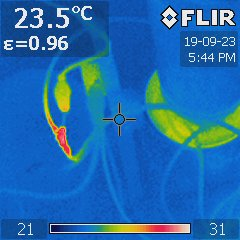
\includegraphics[width=0.5\textwidth]{junctionheat2.jpg}
    \caption{Infrared camera photo of motor during force experiment. The barbed T-junction electrode, seen on the left, heated up rapidly. The circular green region on the right were the motors.}
    \label{fg:tjunction}
\end{figure}

The heat dissipation of the motor without wire circulation was quite poor, but not necessarily worse than other motors with similar designs. As expected, the coil in the motor heated up uniformly, while coils around the edge of the motor, seen in figure \ref{fg:afterexperiment} as yellow, cooled down faster.
\begin{figure}[h!]
    \centering
    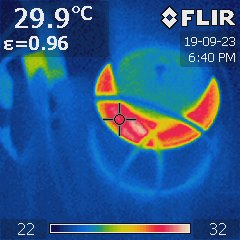
\includegraphics[width=0.5\textwidth]{coilheat.jpg}
    \caption{Infrared camera photo of motor after force experiments. Heat dissipated  slowly from wires.}
    \label{fg:afterexperiment}
\end{figure}

Resistance across the motor from tungsten to tungsten was 0.259 $\Omega$, as measured using a four-wire ohmmeter. 0.187 $\Omega$ was expected of 8 m wire at 2 mm diameter, so the measurement is in line with expectations. The additional resistance may have been the poor contact on the T-junction electrode between tungsten and eGaIn, which is why it heated up rapidly. The tungsten electrodes and any part of the wire that was squeezed to a narrower diameter may have also increased the resistance. Any air bubbles in the wire tubing may also have decreased the effective cross sectional area of the wire in parts, increasing the resistance at that point.

Safety, though not as large of a concern as using mercury or Na-K alloys, is a concern. eGaIn is very corrosive to most metals, and is known to rapidly attack aluminium in particular \cite{cuiLiquidMetalCorrosion2018}. This means the construction of any actuator using eGaIn must be contained and kept away from most tools. The design above addressed this issue by containing the eGaIn in silicone and acrylic. eGaIn is not known to erode tungsten, making it a valid electrode. Carbon-based conductors such as graphite are also not known to corrode via eGaIn, and may be suitable for use in the future. Due to its corrosive properties eGaIn presents a contamination hazard for equipment in the lab and other parts being made in the lab. Care was taken to the best of abilities to minimise the risk of actual contamination, but containment and poisoning procedures of eGaIn are not well established, and require future research before it can be used at commercial scale.

\section{Future Work}
The motor is not currently deformable. A solution is required to create magnetically conductive, if not permanently magnetic core and shell. One possible pathway was explored by Do et al. in \cite{doMiniatureSoftElectromagnetic2018}. However, both the physical and magnetic properties of magnetically-infused silicone are less than ideal as evidenced by the properties testing done in \cite{valentaMechanicalElectricalTesting2008}. The properties of solids that are either magnetic, conductive, or magnetically conductive will inevitably change with deformation. In the case of \cite{valentaMechanicalElectricalTesting2008}, the change in electrical properties as the silicone was deformed was not linear, further complicating the issue.

Another pathway was explored by Lazarus et al. in their recent paper \cite{lazarusCreating3DPrinted2019}, using ferrofluid in 3D printed magnetic devices. Ferrofluid used in their paper had a relative permeability of 19.6, which is an order of magnitude lower than steel, but enough to construct an effective magnetic circuit \cite{ferrotecFerrotecFerrofluidInnovating2019}. It is unclear how the ferrofluid performs under different temperature and pressure conditions. However, it is theoretically possible to construct a fully deformable motor using eGaIn and ferrofluid.

For its magnet, a fully deformable motor can use either a magnetically-infused silicone rod or eGaIn coiled and ferrofluid cored electromagnet. Using the silicone rod will introduce complicated property changes, while using the electromagnet increases power consumption and adds air space which reduces the efficiency.

Custom body for higher fill factor will also most likely be needed, especially for miniaturisation. Fill factors using commercially available tubing will most likely be too low to produce an effective motor at small size.

Controlled circulation of eGaIn in wires and cooling of eGaIn externally will also need to be tested to validate the concept of coil circulation cooling. External cooling presents the challenge that eGaIn is corrosive against most common heat exchanger materials such as copper and aluminium. A heat exchanger made from exotic materials such as tungsten or carbon may be required to successfully circulate cool a liquid metal motor.

\newpage

\section{Conclusion}
A functional voice coil motor that uses liquid eutectic gallium-indium alloy was successfully designed, built and characterised. The motor achieved very similar efficiency to the model calculations from the design and was about 5 - 10 times less power efficient than a motor of the same design and dimensions wired using copper. The design incorporated features that allow for circulation of the liquid metal in the wire for cooling externally to the motor.

Several challenges remain. The motor is not fully deformable and there is no available mechanism to cool circulated eGaIn from the motor. The circulation mechanism also remains untested.

Despite these challenges, this report demonstrates a strong foundation for future investigations into liquid metal wired motors.

\newpage

\printbibliography

\end{document}
